\documentclass{article}
\usepackage{tikz}
\usepackage{hyperref}
\usepackage{apacite}
\usepackage{float}
\usepackage[margin=1in]{geometry}
\usepackage{setspace}
\usepackage{adjustbox}
\usepackage{multirow}
\usepackage[T1]{fontenc} % for smaller printing smaller than sign correctly in plots
\usepackage[labelfont=bf]{caption} % for captions
\usepackage[toc]{appendix} % toc to show in table of contents
\usepackage{tabularx} % expanding tables
\usepackage{amsmath} % Align equations
\usepackage{booktabs} % toprule etc..
\setstretch{1.5}
\pagecolor{white}

\title{Cross-sectional predictability of stock returns in Nordic stock markets using machine learning methods}
\author{Jesse Keränen}
\date{\today}

%add time period to all plot and tables once final

\begin{document}
\maketitle

\thispagestyle{empty}

\newpage

\tableofcontents

\newpage

\section{Introduction}

%In 1808 world was in many ways different compared to what it is today. In 1808 Napoleon was the Emperor of the French Empire and Maximilian I was the King of Kingdom of Bavaria. In 1808 Finnish war broke between Kingdom of Sweden and the Russian Empire which would ultimately lead to establishment of autonomous Grand Duchy of Finland. It would still take more than 100 years for Finland to gain its independence. Same year began the Dano-Swedish war between Sweden and Denmark-Norway. Something historically far less remarkable, but essential for this study happened in 1808 as well. First stock exchange in a Nordic country was opened in Copenhagen. Slowly after that rest of the Nordic countries would open their own stock exchanges as well. Upon facilitated change of ownership of assets, investors were left with a question how to price these assets.

%Major breakthrough in this topic happened when capital asset pricing model was developed in the sixties (sharpe, treynor etc...). In the eighties persofrmance of capital asset pricing model was questioned and scholars came up with so called stock market factors (Earnings-to-price = Basu(1977), Earnings-to-price = Basu(1977), Profitability = e.g., Basu, 1983). During these time machine learning gained large interest and artificial neural networks were popularized. Next big step in asset pricing happened when Eugene Fama and Kenneth French combined these factors to three factor asset pricing model (fama french 1993). Two years after that machine learning method called random forest was introduced (Ho in 1995). Although three factor model was remarkable improvement compared to capital asset pricing model it was not able to explain variation in stock returns completely. In recent years lot of research has applied machine learning methods to capture abnormal returns in stock markets. 

%Nordic market introduction
Objective of this study is to apply set of machine learning methods to well established asset pricing factors to capture abnormal stock return patterns. This study will focus on four Nordic stock markets namely Denmark, Finland, Norway and Sweden. These four markets are relatively homogenous in many aspects. They are geographically close, politically stable and economically interconnected. Denmark, Finland and Sweden all belong to European union. Additionally, stock exchanges of all these three countries are operated by Nasdaq. Therefore, investors could view them as a single market. Some of the features that are characteristic for Nordic markets make them fertile ground for stock market anomaly studies. As mentioned Nordic countries are geographically closely located in northern Europe and therefore relatively distant from large European and especially American markets. European market integration is emphazised by Fama and French \citeyear{FAMA2012457}. 

So called periphery effect has been studied by the scholars a lot. %references)
It refers to investor behaviour where during times of a crisis investors tend to liquidate their investments first from the markets more distant to them. This increases the volatility of periphery markets and can challenge the efficient market theory. Another common feature that Nordic markets share is a high level of foreign ownership. Share of foreign investments in Nordic stock markets can reach more than 50\% \footnotemark. Given the remote location of Nordic stock markets and their high share of foreign ownership it is likely that Nordic countries could be subject to periphery effect. Which again can result abnormal returns.

%all developed, but small -> liquidity

Structure of this paper goes as follows. In second chapter introduction to related literature is provided. In this chapter performance of different methods and persistence of different anomalies in different regions is discussed. Third chapter introduces the methodology and data. Fourth chapter presents the empirical study and final chapter provides as conclusion.

\footnotetext{Butt and Hogholm \citeyear{ButtHogholm2020} calculate share of foreign ownership from IMF Coordinated Direct Investment Survey CDIS data. Foreign ownership share of Butt and Hogholm is 52\% for Denmark, 42\% for Finland, 35\% for Norway and 56\% for Sweden. %check the source
}

\section{Literature}
Being the largest and most prominent stock market in the world US stock market has been subject to majority of asset pricing studies. Despite the dominance of US markets in capturing the the attraction of the academics lot of anomaly asset pricing literature has been conducted in international setting as well. Characteristic for international asset pricing literature is that instead of focusing on single countries they aggregate stock market data to a certain regional level such as Europe or Asia-Pacific. Following chapter provides an overview for pioneering asset pricing anomaly literature. Focus will mainly be on literature on US and European markets. US stock markets are chosen because of their significance on international stock markets and because most anomalies have been discovered there and therefore majority of the initial studies of these anomalies have been conducted there. European studies provide interesting perspective since in many of them Nordic countries are included. 

Chapter introduces the most important anomalies in these markets and how they have been exploited with different methods. This works as starting point to define set of factors that will be used in this study. It can be argued that this kind of process when the set of variables are chosen based on their performance in previous studies is one sort of forward looking information if we try to mimic investors information set. On the other hand Jacobs and Müller \citeyear{JACOBS2020213} only find reliable post-publication decline in long/short returns in US which emphasizes the practical potential of this study.

\subsection{US stock market anomalies}

Many of the recent cross-sectional stock return studies use framework of Lewellen \citeyear{lewellen2015} as base model. He runs 10-year rolling Fama-MacBeth regressions using lagged firm characteristics to predict out of the sample stock returns. He studies cross-sections of US stock return between 1964 and 2013 using different model settings up to 15 company characteristics. He finds strong positive correlation between expected return derived from rolling Fama-MacBeth regressions and realised returns. Additionally Lewellen shows that spread between realised return of portfolio formed from stock with lowest expected returns and portfolio with highest expected return is up to 2.36\%. In his study logarithmic market value of equity, logarithmic book-to-market value, momentum and accruals show the strongest statistical power in explaining monthly returns using lagged variables.

Gu, Jelly and Xiu \citeyear{guetal} contribute to the literature by applying machine learning methods to exploit stock market anomalies. By deploying sophisticated models that do not suffer from over parameterization as heavily as OLS Gu et al. are able to include 94 stock characteristics and their interactions as well as eight aggregated time series variables to their models. Gu et al. use large variety of statistical methods including linear regression, generalized linear models with penalization, dimension reduction via principal components regression and partial least squares, gradient boosted regression trees, random forest and different settings of neural networks. Out of these gradient boosted regression trees and neural networks \footnotemark explain the monthly out of sample stock return the best reaching out of sample $R^{2}$ 0.33 and 0.44 correspondingly where as three factor OLS model introduced by Lewellen \citeyear{lewellen2015} only reaches out of sample $R^{2}$ of -3.46. 

\footnotetext{Gu et al. \citeyear{guetal} use five different settings of neural networks differing by number of hidden layers. Neural network with three hidden layers reaches the highest $R^{2}_{oos}$ and is reported here.}

Similar to Lewellen \citeyear{lewellen2015} Gu et al. construct portfolios based on predicted return of different models. Monthly spread in realized return between portfolio constructed from decile of companies with lowest expected return and decile of stocks with highest expected return \footnotemark is 0.94, 1.62 and 2.12 for models based on OLS, random forest and three layer neural network correspondingly. Gu et al. also show that all methods they examine show somewhat similar patterns on variable importance on return predictability. Most important factors are price trends such as momentum followed by stock liquidity, stock volatility, and valuation ratios.
% all stocks, confirm again
% Deeper neural networks seem to be too complex

\footnotetext{Portfolio returns are average value weighted returns.}

\subsection{European stock market anomalies}

As mentioned US market environment is different in my ways compared to Nordic markets. Fortunately lot of stock market studies have been conducted in Europe and since Nordic markets are usually just a subset of European markets it can be beneficial to have a look on European studies. Tobek and Hronec \citeyear{TOBEK2021100588} study machine learning based anomaly strategies in international setting. Their study includes 153 different equity anomalies and they only include anomalies to their data after documented discovery of corresponding anomaly. This way they can mimic the information set investor would have had and avoid forward looking information. Tobek and Hronec examine five different models including weighted least squares, penalized weighted least squares, gradient boosting regression trees, random forest and neural networks. Their data set spans from 1990 to 2018. Similar to Gu et al. \citeyear{guetal} in US, Tobek and Hronec find that strategy using neural networks provides highest returns on quintile long-short portfolios. Mean return for neural network long-short portfolio in Europe was 0.7. Interestingly penalized weighted least square method provided mean return of 0.651 which is higher than return of random forest based portfolio's return of 0.396. Tobek and Hronec find that Industry momentum, lagged momentum, liquidity shocks, 52 week high, book-to-market value and return on equity are the most important variables for neural networks model.\footnotemark

\footnotetext{Tobek and Hronec \citeyear{TOBEK2021100588} discover possibilities training models either only using historical data from US, using historical data from local markets or using international historical data. Only results for models trained using local data are reported here because that is closest to the setting of this study. Additionally, Tobek and Hronec state that difference between model trained on US data and local data are small.}

Exploiting stock market anomalies using machine learning methods is also studied by Drobetz and Otto \citeyear{Drobetz}. Their data set contains all companies listed in at least one of the 19 Eurozone countries on December 2020 and spans form 1990 to 2020 \footnotemark. Drobetz and Otto examine performance of ordinary least squares, penalized least squares, principal components regressions, partial least squares, random forests, gradient boosted regression trees and neural networks on predicting monthly stock level return exploiting a set of 22 predictions, their two-way interactions and second- and third-order polynomials. Findings of Drobetz and Otto are similar to Gu et al. \citeyear{guetal}. They show that with large number of explanatory variables simple linear regression is not able to explain out of the sample stock returns. 

\footnotetext{Finland is the only country included in the study of Drobetz and Otto \citeyear{Drobetz} that is also included in this study, since it is the only country belonging to Eurozone.}

Findings of Drobetz and Otto \citeyear{Drobetz} are also similar to Tobek and Hronec \citeyear{TOBEK2021100588} in a sense that least squares methods where dimensionality is restricted can actually perform better than tree based methods. Like in majority of other literature, Drobetz and Otto find out that neural networks provide superior framework for stock return prediction model measured in both explanatory power and profitability. Neural network method reaches out of the sample $R^{2}$ value of 1.23 and long-short portfolio formed based on expected returns derived from neural networks model provide average value weighted monthly return of 1.94\%. Similar to Gu et al. \citeyear{guetal} Drobetz and Otto find that same variables show the most importance across the different models, most notably earnings-to-price ratio and 12 month momentum.
%Deeper neural networks seem to be too complex

Fieberg et al \citeyear{Fieberg} study stock market anomalies in 16 European stock markets using machine learning methods over almost the same period as Drobetz and Otto \citeyear{Drobetz} \footnotemark. Nevertheless they choose a slightly different approach where instead of including vast set of anomalies, they only consider six prominent equity factors. Their conclusion endorses findings of Drobetz and Otto \citeyear{Drobetz} and Tobek and Hronec \citeyear{TOBEK2021100588} as they shown that more complex machine learning models beat linear approach in terms of both economic and statistical performance.

\footnotetext{Dataset of Fieberg et al \citeyear{Fieberg} contains Denmark, Finland, Norway and Sweden}

\subsection{Stock market anomalies in Nordic markets}

This chapter provides an overview of observed stock market anomalies in different Nordic stock markets. Many studies in this chapter have slightly different objective than this study. Studies show the existence of the anomalies by constructing a portfolio heavily weighted on certain factor. Nevertheless, they do not describe the magnitude of the relationship between the factor and the stock returns. This study has slightly more ambitious objective and tries to derive return expectations from predefined stock market factors. This literature review serves as starting point for choosing most promising stock market factors that have already been studied.
%small amount of stocks

Magnitude of value and momentum anomalies in Nordic stock markets are examined in the paper by Grobys and Huhta-Halkola \citeyear{grobys}. They combine information from companies listed in main lists of Danish, Finnish, Norwegian and Swedish stock exchanges between 1991 and 2017. Grobys and Huhta-Halkola measure value with book-to-market value and momentum with past 12-month total shareholder equity%return??? % 
. Grobys and Huhta-Halkola show that momentum effect exists in Nordics markets and profitability of momentum strategy is not related to size factor. Value factor yields also significant excess return, but according to Grobys and Huhta-Halkola it could be partly driven by the size factor, since value premium reduces when accounted for the size. Among all stocks monthly average equally weighted long-short return is 1.73\% and 1.25\% for momentum and value strategies correspondingly. Both of the excess returns are statistically highly significant. Grobys and Huhta-Halkola also test combination strategies using signals from both momentum and strategy which yield even stronger results.

Value premium has shown consistency in Finnish stock markets. Davydov, Tikkanen and Äijö \citeyear{Davydov2017MagicFV} examine profitability of different value investing strategies between 1991 and 2013. Davydov et. al. investigate set of value indicators which included earnings to price, book to price, cash flow to price, dividends to price and earnings before income and taxes to enterprise value ratios. Additionally they test performance of investing strategy developed by Greenblatt (cite here) where portfolios are formed based on combined ranking of company's return on invested capital and earnings before income and taxes to enterprise value ratio. They show that returns of all of the value portfolios not only beat the market return, but can also not be explained by the four factor model of Carhart \citeyear{https://doi.org/10.1111/j.1540-6261.1997.tb03808.x}.  
%(Finnish Stock Exchange in the period 1991–2013. In total, the number of companies varies from 39 to 136)
%check the second article from patari and leivo

Similar to Grobys and Huhta-Halkola \citeyear{grobys} Leivo and Pätäri \citeyear{cite-key} combine value anomaly with momentum anomaly in Finnish stock market for data set between 1993 and 2008. They show that two step portfolio sort that first allocates stocks to three portfolios based on their value indicators and subsequently based on momentum indicator can capture extraordinary stock returns. Leivo and Pätäri show that including momentum further increases returns of already recognised value sorting. Strategy performs even better when authors allow for long position in high value high momentum portfolio and short position on low value low momentum portfolio. Excess returns resulting from the two-fold portfolio construction can not be explained by CAP-model or two factor model including also size factor. It is not a surprise that value and momentum premium show existence in Nordic markets. Value and momentum anomalies are among the most well documented factors showing persistence in multiple cross-sectional studies (e.g, Gu, Jelly and Xiu \citeyear{guetal}, Lewellen \citeyear{lewellen2015}, Drobetz and Otto \citeyear{Drobetz}, Tobek and Hronec \citeyear{TOBEK2021100588} ).
% Helsinki Stock Exchange (HEX; later OMX Helsinki) during the period 1993–2008. E/P, EBITDA/EV, CF/P, dividend yield (D/P), B/P and S/P and combinations.
%re-phrase the text

Nordic stock markets have several characteristic features. One is that all Nordic stock markets are considered to be developed, but also small. Especially market capitalization of companies listed in Nordic stock exchanges are on average much smaller than in US. Therefore, it is reasonable to ask whether liquidity of the stock could be driving factor of the stock returns. Impact of illiquidity risk to stock returns in Nordic market setting has been studied by Butt and Hogholm \citeyear{ButtHogholm2020}. Butt and Hogholm test variety of different illiquidity measures and find that dollar zero returns is the most profitable illiquidity anomaly measure across all four Nordic market. Dollar zero return measurement is calculated by dividing number of days stocks return in US dollars is zero by total number of trading days. Butt and Hogholm construct five quintile portfolios based on liquidity of the stocks with data spanning from 1988 to 2013. They show that in all Nordic markets there exists large illiquidity premium as annual difference in equal weighted return of most illiquid portfolio and least illiquid portfolio is more than 18\% for Finland, Norway and Sweden. For Denmark premium is slightly smaller 8.8\%.

Jokipii and Vähämaa \citeyear{jokipii2006free} investigate free cash flow anomaly in Finnish stock markets between 1992 and 2002. They construct portfolios from stocks listed in Finnish stock exchange based on predefined thresholds for free cash flow ratios. These ratios include market value to free cashflow and total debt to free cashflow ratios. High free cashflow portfolio yields higher returns than market on average and the excess returns can not be completely explained by weightings in Fama and French \citeyear{FAMA19933} risk factors.
%Finnish companies during the period 1992-2002. net cash flow from operating activities minus capital expenditures. The net cash flow from operating activities, in turn, is defined as the sum of net income, all non-cash charges and credits (e.g.,  depreciation,  amortization  of  intangibles,  and  deferred  taxes),  extra ordinary items, and net change in working capital

\section{Data}
Main datasource for this study is Thomson Datastream. Company fundamental data is collected from Worldscope. Dataset spans from 1990 January to 2022 December which is shorter than in many previous studies. Reason why time period is limited to 1990 is that amount of publicly listed companies in Nordic markets was rather low in the 1980's and finding reliable data for period before 1990 is difficult. Dataset contains all stocks listed in primary markets of corresponding countries including also companies that went bankrupt or were de-listed for any other reason. Therefore dataset is not subject to survivorship bias. Panel A of table \ref{table:markets} in Appendix shows the constituent lists used in data collection. As highlighted by Ince and Porter \citeyear{Ince2006} data in Datastream can be noisy and uncleaned data could lead to a false statistical inference. Therefore several static and dynamic screens are applied to the data. Screens include filtering non-equity securities, securities that are not listed in respective country and securities that are quoted in currency other than respective country's currency. All applied static and dynamic screens are comprehensively explained in appendix. 

\begin{table}[h] 
\caption{\textbf{Country summary statistics}\\ Table provides summary statistics for pooled Nordic market and separate country specific Nordic markets. Minimum number of companies tells the amount of companies included to the data set in a month that the value was lowest for respective country. Maximum number of companies tells the amount of companies included to the data set in a month that the value was highest for respective country. Mean number of companies is the time series average of monthly number of companies for each country. Total number of companies is the number of unique companies in whole data set. Time series averages for monthly mean, median and total market values are also presented. Total market value is sum of market values of respective country in each month. All marked values are converted to USD. Only companies in the final dataset are included in calculation of the figures.}
 \label{table:CountrySummary}
\centering
\newcolumntype{Y}{>{\raggedleft\arraybackslash}X}
\begin{tabularx}{\textwidth}{@{\extracolsep{4pt}} X Y Y Y Y Y Y Y} 
\toprule
 & \multicolumn{4}{c}{Number of companies} & \multicolumn{3}{c}{Market value} \\
\cline{2-5} \cline{6-8} 
	 		& Min 	& Max 	& Mean  	& Total	& Mean 		& Median 	& Total \\
\midrule
Denmark	 	& 60 		& 124 	& 96 		& 216	& 1726.66 	& 99.95	& 170315.4  \\
Finland	 	& 32 		& 120 	& 96 		& 186 	& 2117.73 	& 250.64	& 174166.7  \\
Norway		& 43 		& 149 	& 100 	& 304	& 1301.29 	& 172.69  & 136871.4 \\
Sweden		& 39 		& 506 	& 266 	& 784	& 1414.79 	& 133.72	& 342283.2  \\
\midrule
Nordic		& 193 	& 873 	& 558 	& 1490	& 1362.78 	& 131.55 	& 760958.3  \\
\bottomrule
\end{tabularx}
\end{table} 

The number of stocks in the dataset is 873 where as the monthly number of stocks in the dataset is 558 on average. Figure \ref{plot:number_of_companies} in Appendix shows the development of the company count that passed the statistical screens over time. Table \ref{table:CountrySummary} on the other hand includes only companies included in the final dataset which requires that there was no missing information for the company in respective month \footnotemark. By comparing the figure \ref{plot:number_of_companies} and the table \ref{table:CountrySummary} it can be seen that number of companies in the dataset is mainly limited by the availability of the company characteristics data, especially in the beginning of the time period. Sweden is clearly the biggest of the four markets both in regards of the number of companies and total market value of the companies. Size characteristics of rest of the countries are quite homogenous.

\footnotetext{For certain variables missing information is treated as zero.}
% Update this list once final

\begin{table}[ht] 
\caption{\textbf{Descriptive statistics}\\ Table provides time series average of cross-sectional means and standard deviations of all variables used in this study. Values are reported separately for pooled Nordic market and four Nordic markets Denmark, Finland, Norway and Sweden. RET is monthly return calculated from total return index.}
 \label{table:descriptive}
\centering
\begin{tabularx}{\textwidth}{@{\extracolsep{4pt}} X r r r r r r r r r r} 
\toprule
 & \multicolumn{2}{c}{Nordic} & \multicolumn{2}{c}{Denmark} & \multicolumn{2}{c}{Finland} & \multicolumn{2}{c}{Norway}&\multicolumn{2}{c}{Sweden} \\
\cline{2-3}\cline{4-5}\cline{6-7}\cline{8-9}\cline{10-11}
Variable 		& Mean 	& Std. & Mean & Std. & Mean & Std. & Mean & Std. & Mean & Std. \\
\midrule
RET			& 0.0130 	& 2 & 3 & 4 & 5 & 6 & 7 & 8 & 9 & 10 \\
Cash/Asset 	& 0.1587 	& 2 & 3 & 4 & 5 & 6 & 7 & 8 & 9 & 10 \\
CapTurnOver 	& 1.0432 	& 2 & 3 & 4 & 5 & 6 & 7 & 8 & 9 & 10 \\
INV 			& 0.6598 	& 2 & 3 & 4 & 5 & 6 & 7 & 8 & 9 & 10 \\
BEME 		& -2.2394 & 2 & 3 & 4 & 5 & 6 & 7 & 8 & 9 & 10 \\
CF/Price 		& 0.0410 	& 2 & 3 & 4 & 5 & 6 & 7 & 8 & 9 & 10 \\
Leverage 		& 0.7644 	& 2 & 3 & 4 & 5 & 6 & 7 & 8 & 9 & 10 \\
Sales/Price 	& 1.1321 	& 2 & 3 & 4 & 5 & 6 & 7 & 8 & 9 & 10 \\
E/P 			& -0.0302 & 2 & 3 & 4 & 5 & 6 & 7 & 8 & 9 & 10 \\
ROA 		& -0.0079 & 2 & 3 & 4 & 5 & 6 & 7 & 8 & 9 & 10 \\
ROE 		& 0.2033 	& 2 & 3 & 4 & 5 & 6 & 7 & 8 & 9 & 10 \\
MOM$_{7}$ 	& 0.0829 	& 2 & 3 & 4 & 5 & 6 & 7 & 8 & 9 & 10 \\
MOM$_{12}$ 	& 0.1782 	& 2 & 3 & 4 & 5 & 6 & 7 & 8 & 9 & 10 \\
MOM$_{24}$ 	& 0.3908 	& 2 & 3 & 4 & 5 & 6 & 7 & 8 & 9 & 10 \\
MOM$_{2}$ 	& 0.1714 	& 2 & 3 & 4 & 5 & 6 & 7 & 8 & 9 & 10 \\ 
\bottomrule
\end{tabularx}
\end{table} 

Total X characteristics are derived from stock level data. All the models use same set of explanatory variables which includes cash flow-to-total assets ratio, capital turnover, investment, book-to-market ratio, cashflow-to-price ratio, leverage, sales-to-price ratio, earnings-to-price ratio, return on assets, return on equity and 2, 7, 12 and 24 month momentum. Detailed descriptions how each of these variables is calculated is provided in the table \ref{table:variableDefs} in appendix. Majority of these variables are calculated from income statement or balance sheet information and therefore updated only once a year. To account for possible reporting delay associated with accounting data, accounting data from year $t$ is considered to be available end of June $t+1$. Table \ref{table:descriptive} provides descriptive statistics of company characteristics. Descriptive statistics are reported for pooled nordic markets as well as individual markets.

\section{Methodology}
This study will evaluate tested methods from two perspectives. Both of them depend on expected returns provided by the methods. How different methods derive the expected returns is explained in the following subsections. First more economical perspective is how profitable predictions of different models would have turned out to be. Profitability is estimated via portfolio construction following Lewellen \citeyear{lewellen2015}. Each month based on the expected return produced by the model all stocks are allocated to quintile portfolios. Object of the interest is the spread between lowest and highest expected return portfolios. Both value and equal weighted returns will be reported for each portfolio. Long-short returns will be calculated from the returns of portfolio with highest and lowest expected returns. These returns will be regressed agains Fama-French \citeyear{FAMA19933} three factor model factors to test if model was able to produce returns that can not be explained with loadings of Fama and French risk factors.

Second more statistical measure is how precise prediction methods was able to produce. Prediction accuracy will be evaluated using out-of-smaple $R^{2}_{oos} $ from (source). 

\begin{equation}
\label{eq:r2}
R^{2}_{oos} = 1 - \frac{\sum^T_{t=1} \sum^N_{i=1} (r_{i, t} - \hat r_{i, t})^2}{ \sum^T_{t=1} \sum^N_{i=1} r^2_{i, t}}
\end{equation}

Factors importance

\subsection{Linear regression}
Benchmark model of this study is Fama-MacBeth \citeyear{FamaMacBeth1973} regression. First step of the method is to run rolling cross-sectional regressions with lagged variables. Second step of the method calculates means of the factor loadings obtained from the cross-sectional regressions. Finally expected stock return can be obtained by multiplying the mean factors loading with latest available stock characteristics. Below formulas show one model specification for Fama-French \citeyear{FAMA19933} three factors model.

\begin{equation}
r_{i, t} = \beta_0 + \beta_{1,t} \ Mkt_{i, t-1} + \beta_{2, t} + \ Size_{i, t-1} + \beta_{3, t} \ Value_{i, t-1} + \epsilon_{i}
\end{equation}

\begin{equation}
\overline \beta_j = \frac{1}{T} \sum^{T}_{t=1}\beta_{j, t}
\end{equation}

\begin{equation}
E(r_{i, t}) = \overline \beta_0 + \overline \beta_{1, t} \ Mkt_{i, t-1} + \overline \beta_{2, t} + \ Size_{i, t-1} + \overline \beta_{3, t} \ Value_{i, t-1}
\end{equation}

One benefit that linear regression models have is that they do not require hyperparameter tuning. Therefore data  does not have to be split to three sub-samples for separate validation of hyperparameters and testing. To obtain the expected return mean of 120 historical regression coefficients is calculated. Due to their high computing cost machine learning models are usually trained only once a year and then used for the rest of the year. Each month recent information is just inserted to the model. Computing requirements for linear model is far lesser than for non-linear models. Nevertheless to ensure comparability between different models also the linear model is trained only once per year. That means that no more recent stock returns than $t-1$ are used to train the model to predict stock return $t$, but the gap between predicted return and last return used to train the model can grow up to 12 months. Since we use lagged variables, this means that for prediction of stock return $t$ we alway use stock characteristics from $t-1$, but some factors are only updated yearly. To mimic information set investor would have had available in historical periods we have to account for the delay in reporting balance sheet information. Therefore timeline of Fama and French \citeyear{FAMA19933} is followed and models are trained each year at end of June. 

\subsection{Random forest}
Decision trees are one example of nonparametric machine learning algorithms. Idea of the decision trees is to split data into the most homogenous groups. Starting point of the regression tree is called a root node. At each iteration of regression tree algorithm finds the optimal threshold to split the data to the nodes to minimize objective function. Then iteratively these nodes can be further split and the tree grows. This process is repeated until predefined tree size, set by the user, is reached or objective function can not be improved anymore. Regression tree nodes that are not further split are called leaves. Final prediction of the regression tree leaf is the average of the dependant variable values of training set observations inside it. Gu et al. \citeyear{guetal} formulate prediction of a regression tree with $K$ leaves as 

\begin{equation}
f(x_{i, t}; \theta, K, L) = \sum_{k=1}^K \theta_k 1 _{\{x_{i, t} \in C_K(L)\}}
\end{equation}

Where $C_k(L)$ represents one of the $K$ splits the tree consists of. $L$ is the indicator of the depth of the leaf. $\theta_k$ indicates average return within leaf $k$ and $1 _{\{x_{i, t} \in C_K(L)\}}$ indicates whether observation $x_{i, t}$ belongs to leaf $k$. Since observation can only belong to one leaf, partition $C_K(L)$ is the product of the above partitions.

\begin{figure}
\centering
\caption{\textbf{Illustrative regression tree}\\ Tree is trained from the actual dataset for 30th of July 2004 and then pruned to show only few most important leaves. Figure serves only illustrative purposes and random forest models used in the study do not necessarily contain identical trees. }
% Created by tikzDevice version 0.12.6 on 2024-02-09 09:47:03
% !TEX encoding = UTF-8 Unicode
\begin{tikzpicture}[x=1pt,y=1pt]
\definecolor{fillColor}{RGB}{255,255,255}
\path[use as bounding box,fill=fillColor,fill opacity=0.00] (0,0) rectangle (289.08,289.08);
\begin{scope}
\path[clip] ( 49.20, 61.20) rectangle (263.88,239.88);
\definecolor{drawColor}{RGB}{0,0,0}

\node[text=drawColor,anchor=base,inner sep=0pt, outer sep=0pt, scale=  1.00] at (156.54,230.76) {|};

\path[draw=drawColor,line width= 0.4pt,line join=round,line cap=round] ( 86.97,178.11) --
	( 86.97,233.26) --
	(226.11,233.26) --
	(226.11,178.11);

\path[draw=drawColor,line width= 0.4pt,line join=round,line cap=round] ( 57.15,122.97) --
	( 57.15,178.11) --
	(116.78,178.11) --
	(116.78,122.97);

\path[draw=drawColor,line width= 0.4pt,line join=round,line cap=round] ( 96.91, 67.82) --
	( 96.91,122.97) --
	(136.66,122.97) --
	(136.66, 67.82);

\path[draw=drawColor,line width= 0.4pt,line join=round,line cap=round] (196.30,122.97) --
	(196.30,178.11) --
	(255.93,178.11) --
	(255.93,122.97);

\path[draw=drawColor,line width= 0.4pt,line join=round,line cap=round] (176.42, 67.82) --
	(176.42,122.97) --
	(216.17,122.97) --
	(216.17, 67.82);
\end{scope}
\begin{scope}
\path[clip] (  0.00,  0.00) rectangle (289.08,289.08);
\definecolor{drawColor}{RGB}{0,0,0}

\node[text=drawColor,anchor=base,inner sep=0pt, outer sep=0pt, scale=  0.70] at (156.54,236.99) {L.BETA>=1.198};

\node[text=drawColor,anchor=base,inner sep=0pt, outer sep=0pt, scale=  0.70] at ( 86.97,182.04) {L.HIGH52.RATIO< 0.7105};

\node[text=drawColor,anchor=base,inner sep=0pt, outer sep=0pt, scale=  0.70] at (116.78,126.90) {MOM12< 0.6632};

\node[text=drawColor,anchor=base,inner sep=0pt, outer sep=0pt, scale=  0.70] at (226.11,182.04) {MOM36< -0.06951};

\node[text=drawColor,anchor=base,inner sep=0pt, outer sep=0pt, scale=  0.70] at (196.30,126.90) {MOM7< 0.1648};

\node[text=drawColor,anchor=base,inner sep=0pt, outer sep=0pt, scale=  0.70] at ( 57.15,118.76) {-0.1218};

\node[text=drawColor,anchor=base,inner sep=0pt, outer sep=0pt, scale=  0.70] at ( 57.15,110.36) {n=14};

\node[text=drawColor,anchor=base,inner sep=0pt, outer sep=0pt, scale=  0.70] at ( 96.91, 63.61) {-0.08305};

\node[text=drawColor,anchor=base,inner sep=0pt, outer sep=0pt, scale=  0.70] at ( 96.91, 55.21) {n=32};

\node[text=drawColor,anchor=base,inner sep=0pt, outer sep=0pt, scale=  0.70] at (136.66, 63.61) {-0.0333};

\node[text=drawColor,anchor=base,inner sep=0pt, outer sep=0pt, scale=  0.70] at (136.66, 55.21) {n=21};

\node[text=drawColor,anchor=base,inner sep=0pt, outer sep=0pt, scale=  0.70] at (176.42, 63.61) {-0.1258};

\node[text=drawColor,anchor=base,inner sep=0pt, outer sep=0pt, scale=  0.70] at (176.42, 55.21) {n=9};

\node[text=drawColor,anchor=base,inner sep=0pt, outer sep=0pt, scale=  0.70] at (216.17, 63.61) {-0.03391};

\node[text=drawColor,anchor=base,inner sep=0pt, outer sep=0pt, scale=  0.70] at (216.17, 55.21) {n=26};

\node[text=drawColor,anchor=base,inner sep=0pt, outer sep=0pt, scale=  0.70] at (255.93,118.76) {-0.007807};

\node[text=drawColor,anchor=base,inner sep=0pt, outer sep=0pt, scale=  0.70] at (255.93,110.36) {n=216};
\end{scope}
\end{tikzpicture}

\label{plot:regre_tree}
\end{figure}

Advantage of the regression trees is that they are are rather simple and intuitive, but still they are able to model even complex interactions among predictors and non-linear relationships. One common problem with regression trees is that they easily overfit the data and would require heavy regularization. Random forest models aims to avoid this problem by deriving the predictions from ensemble of regression trees.

\subsection{Neural networks}

\appendix
\section{Data}
\renewcommand{\thefigure}{A.\arabic{figure}}
\setcounter{figure}{0}
\renewcommand{\thetable}{A.\arabic{table}}
\setcounter{table}{0}

\begin{table}[H] 
\caption{\textbf{Constituent lists and keywords}\\ Table provides the constituent lists used in data collection.}
 \label{table:constituteLists}
\centering
\begin{tabularx}{\textwidth}{X X X X}
\toprule
Denmark & Finland & Norway & Sweden \\
\midrule
FDEN 		&  FFIN		& FNOR		& FSWD\\
WSCOPEDK & WSCOPEFN & WSCOPENW& WSCOPESD\\
DEADDK 	&   DEADFN 	& DEADNW 	& DEADSD\\
& & & FAKTSWD\\
 \bottomrule
 \end{tabularx}
 \end{table} 

 \begin{table}[h]
\caption{\textbf{Static screens}\\ It also provides the country specific keywords that are used to deleted entries from the dataset. Panel B provides keywords that were used to delete entries from each market separately. Keyword deletion follows Ince and Porter \protect\citeyear{Ince2006} and Hanauer and Windmüller \protect\citeyear{HANAUER2023106712}. Same logic is applied to remove both country specific and generic keywords. Keyword is searched from Datastream attributes NAME, ENAME and ECNAME. In case if at least one of these attributes contains the keyword security is deleted from the dataset. To avoid deleting proper entries, security is only deleted if keyword occurs at the beginning of the name, at the end of the name or as separate word in the name.}
\label{table:staticscreens}
\begin{tabularx}{\textwidth}{X X X X l}
\toprule
\multicolumn{5}{l}{\textit{Panel A: Static screens.}} \\
\midrule
 & Denmark & Finland & Norway & Sweden\\
\midrule
MAJOR & Y & Y & Y & Y\\
TYPE & EQ & EQ & EQ & EQ\\
ISINID & P & P & P & P\\
GEOGN & DENMARK & FINLAND & NORWAY & SWEDEN\\
GEOLN & DENMARK & FINLAND & NORWAY & SWEDEN\\
PCUR & DK & FI, MK & NK & SK\\
GGSIN & DK & FI & NO &SE\\
\toprule
\multicolumn{5}{l}{\textit{Panel A: Country specific keywords.}} \\
\midrule
 & Denmark & Finland & Norway & Sweden\\
 \midrule
NAME & \multirow[m]{3}{*}{ \textbackslash \textbackslash)CSE \textbackslash \textbackslash} & \multirow[m]{3}{*}{USE} & & \multirow[m]{3}{13em}{CONVERTED INTO, USE, CONVERTED-, CONVERTED - SEE}\\
ENAME & & \\
ECNAME & &\\
\bottomrule
\end{tabularx}
\end{table}


\begin{table}[H] 
\caption{\textbf{Country specific keywords}\\ Table shows the general keywords that were used to delete entries from all markets. Keyword deletion follows Ince and Porter \protect\citeyear{Ince2006} and Hanauer and Windmüller \protect\citeyear{HANAUER2023106712}. Same logic is applied to remove both country specific and generic keywords. Keyword is searched from Datastream attributes NAME, ENAME and ECNAME. In case if at least one of these attributes contains the keyword security is deleted from the dataset. To avoid deleting proper entries, security is only deleted if keyword occurs at the beginning of the name, at the end of the name or as separate word in the name.}
 \label{table:generalKeywords}
\centering
\begin{tabularx}{\textwidth}{l X}
\toprule
Security class 	& Keywords \\
\midrule
Duplicates 		& 1000DUPL, DULP, DUP, DUPE, DUPL, DUPLI, DUPLICATE, XSQ, XETa  \\[1ex]
Depository receipts	& ADR, GDR \\[1ex]
Preferred stock 	&  PF, ’PF’, PFD, PREF, PREFERRED, PRF\\ [1ex]
Warrants 			&  WARR, WARRANT, WARRANTS, WARRT, WTS, WTS2\\[1ex]
Debt 			& \%, DB, DCB, DEB, DEBENTURE, DEBENTURES, DEBT\\[1ex]
Unit trusts 		& .IT, .ITb, TST, INVESTMENTTRUST, RLSTIT, TRUST, TRUSTUNIT, TRUSTUNITS, TST, TSTUNIT, TST UNITS, UNIT, UNITTRUST, UNITS, UNT, UNTTST, UT\\[1ex]
ETFs 			& AMUNDI, ETF, INAV, ISHARES, JUNGE, LYXOR, X-TR\\[1ex]
Expired securities 	& EXPD, EXPIRED, EXPIRY, EXPY\\[1ex]
Miscellaneous 		& ADS, BOND, CAP.SHS, CONV, DEFER, DEP, DEPY, ELKS, FD, FUND, GW.FD, HI.YIELD, HIGHINCOME, IDX, INC.								\&GROWTH, INC.\&GW, INDEX, LP, MITS, MITT, MPS, NIKKEI, OPCVM, ORTF, PERQS, 												PFC, PFCL, PINES, PRTF, PTNS, PTSHP, QUIBS, QUIDS, RATE, RCPTS, REALEST, RECEIPTS, REIT, RESPT, 								RETUR, RIGHTS, RST, RTN.INC, RTS, SBVTG, SCORE, SPDR, STRYPES, TOPRS, UTS, VCT, VTG.SAS, 									XXXXX, YIELD,YLD, PF.SHS.\\
 \bottomrule
 \end{tabularx}
 \end{table} 

\begin{table}[H] 
\caption{\textbf{Variable definitions} \\Tables provides definitions and initial authors for all anomalies used in the study. Construction of variables follows Green et. al \protect\citeyear{Green2017} and Hanauer and Kalsbach \protect\citeyear{HANAUER2022}.}
\label{table:variableDefs}
\centering
\begin{tabularx}{\textwidth}{l X X}
\toprule
Variable & Author & Definition\\
\midrule
Cash-to-Assets 		& \cite{PALAZZO2012162} 	& Cash-to-Asset ratio is calculated by dividing  cash and short-term investments by total assets.\\
Capital Turnover 		& & \\
Investment 			& & \\
Book-to-Market Equity 	& \cite{Rosenberg1985} 		&  Book-to-Market value is calculated by dividing company's book value of equity by company's market 										 	capitaliztion end of previous year. Book value of equity is calculated by summing common 												equity and deferred taxes of the company. \\
Cash Flow-to-Price 		& \cite{LAKONISHOK1994} 	& Cash flow to price ratio is calculated by dividing company's cash flow from operating activities 												by asset's market capitaliztion end of previous year. \\
Leverage 				& & \\
Sales-to-Price 			& & Sales-to-price ratio is calculated by dividing total sales by asset's market capitaliztion end of previous year.\\
Earnings-to-Price 		& & Earnings-to-price ratio is calculated by dividing net income before extra Items and preferred dividends by asset's market capitaliztion end of previous year.\\
Return-on-Assets 		& & Return-on-assets is calculated as net income before extra Items and preferred dividends divided by one year lagged total assets.\\
Return-on-Equity 		& & Return-on-equity is calculated as net income before extra Items and preferred dividends divided by one year lagged book value of equity. See book-to-market equity for definition of book value of equity. \\
Momentum$_{7}$ 		& & Cumulative return in US dollars between $t-7$ and $t-12$ months.\\
Momentum$_{12}$ 		& & Cumulative return in US dollars between $t-2$ and $t-12$ months.\\
Momentum$_{36}$ 		& & Cumulative return in US dollars between $t-12$ and $t-36$ months.\\
Momentum$_{2}$ 		& & Prior month return in US dollars.\\ 
\bottomrule
\end{tabularx}
\end{table} 

\begin{figure}[H]
\centering
\caption{\textbf{Number of companies}\\ Figure shows the delopment of total number of securities considered in the dataset from 1990 to 2022 for each Nordic country. Figures counts all securities that passed the static screens. Final amount of companies in each time point can be lower since security will be excluded from the dataset if it is missing certain information.}
% Created by tikzDevice version 0.12.6 on 2024-03-22 10:26:56
% !TEX encoding = UTF-8 Unicode
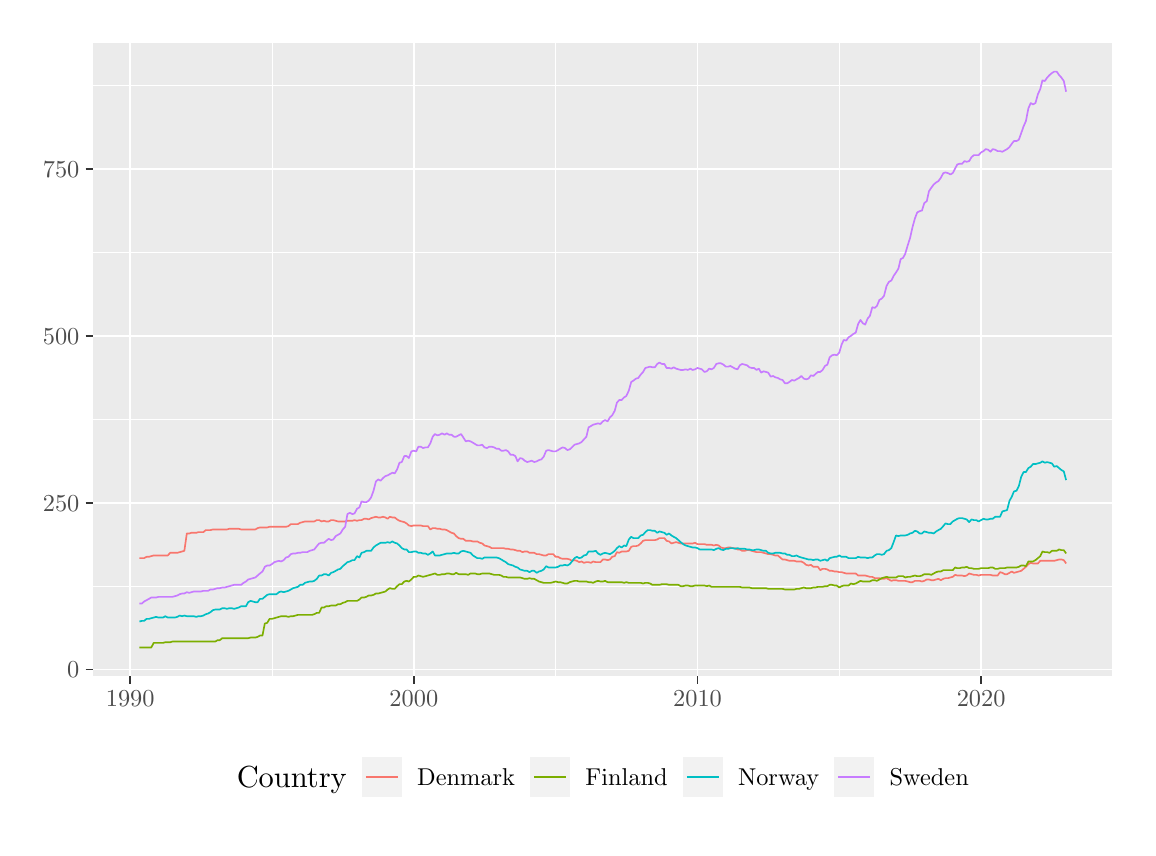
\begin{tikzpicture}[x=1pt,y=1pt]
\definecolor{fillColor}{RGB}{255,255,255}
\path[use as bounding box,fill=fillColor,fill opacity=0.00] (0,0) rectangle (397.48,289.08);
\begin{scope}
\path[clip] (  0.00,  0.00) rectangle (397.48,289.08);
\definecolor{drawColor}{RGB}{255,255,255}
\definecolor{fillColor}{RGB}{255,255,255}

\path[draw=drawColor,line width= 0.6pt,line join=round,line cap=round,fill=fillColor] (  0.00,  0.00) rectangle (397.48,289.08);
\end{scope}
\begin{scope}
\path[clip] ( 23.65, 54.68) rectangle (391.98,283.58);
\definecolor{fillColor}{gray}{0.92}

\path[fill=fillColor] ( 23.65, 54.68) rectangle (391.98,283.58);
\definecolor{drawColor}{RGB}{255,255,255}

\path[draw=drawColor,line width= 0.3pt,line join=round] ( 23.65, 87.26) --
	(391.98, 87.26);

\path[draw=drawColor,line width= 0.3pt,line join=round] ( 23.65,147.55) --
	(391.98,147.55);

\path[draw=drawColor,line width= 0.3pt,line join=round] ( 23.65,207.83) --
	(391.98,207.83);

\path[draw=drawColor,line width= 0.3pt,line join=round] ( 23.65,268.11) --
	(391.98,268.11);

\path[draw=drawColor,line width= 0.3pt,line join=round] ( 88.29, 54.68) --
	( 88.29,283.58);

\path[draw=drawColor,line width= 0.3pt,line join=round] (190.80, 54.68) --
	(190.80,283.58);

\path[draw=drawColor,line width= 0.3pt,line join=round] (293.30, 54.68) --
	(293.30,283.58);

\path[draw=drawColor,line width= 0.6pt,line join=round] ( 23.65, 57.12) --
	(391.98, 57.12);

\path[draw=drawColor,line width= 0.6pt,line join=round] ( 23.65,117.41) --
	(391.98,117.41);

\path[draw=drawColor,line width= 0.6pt,line join=round] ( 23.65,177.69) --
	(391.98,177.69);

\path[draw=drawColor,line width= 0.6pt,line join=round] ( 23.65,237.97) --
	(391.98,237.97);

\path[draw=drawColor,line width= 0.6pt,line join=round] ( 37.05, 54.68) --
	( 37.05,283.58);

\path[draw=drawColor,line width= 0.6pt,line join=round] (139.54, 54.68) --
	(139.54,283.58);

\path[draw=drawColor,line width= 0.6pt,line join=round] (242.05, 54.68) --
	(242.05,283.58);

\path[draw=drawColor,line width= 0.6pt,line join=round] (344.54, 54.68) --
	(344.54,283.58);
\definecolor{drawColor}{RGB}{248,118,109}

\path[draw=drawColor,line width= 0.6pt,line join=round] ( 40.39, 97.39) --
	( 41.26, 97.39) --
	( 42.07, 97.39) --
	( 42.97, 97.87) --
	( 43.84, 97.87) --
	( 44.63, 98.12) --
	( 45.55, 98.36) --
	( 46.40, 98.36) --
	( 47.27, 98.36) --
	( 48.13, 98.36) --
	( 48.92, 98.36) --
	( 49.73, 98.36) --
	( 50.63, 98.36) --
	( 51.50, 99.32) --
	( 52.29, 99.32) --
	( 53.21, 99.32) --
	( 54.06, 99.32) --
	( 54.93, 99.56) --
	( 55.80, 99.80) --
	( 56.61,100.04) --
	( 57.51,106.31) --
	( 58.38,106.31) --
	( 59.16,106.55) --
	( 60.06,106.55) --
	( 60.90,106.55) --
	( 61.72,106.80) --
	( 62.62,106.80) --
	( 63.49,106.80) --
	( 64.36,107.52) --
	( 65.20,107.52) --
	( 66.04,107.52) --
	( 66.91,107.76) --
	( 67.78,107.76) --
	( 68.59,107.76) --
	( 69.38,107.76) --
	( 70.31,107.76) --
	( 71.15,107.76) --
	( 72.02,107.76) --
	( 72.86,108.00) --
	( 73.70,108.00) --
	( 74.60,108.00) --
	( 75.44,108.00) --
	( 76.25,108.00) --
	( 77.15,107.76) --
	( 78.02,107.76) --
	( 78.89,107.76) --
	( 79.68,107.76) --
	( 80.55,107.76) --
	( 81.36,107.76) --
	( 82.26,107.76) --
	( 83.10,108.24) --
	( 83.92,108.48) --
	( 84.84,108.48) --
	( 85.68,108.48) --
	( 86.55,108.48) --
	( 87.40,108.72) --
	( 88.24,108.72) --
	( 89.14,108.72) --
	( 89.92,108.72) --
	( 90.79,108.72) --
	( 91.58,108.72) --
	( 92.50,108.72) --
	( 93.35,108.72) --
	( 94.22,108.97) --
	( 95.09,109.69) --
	( 95.90,109.69) --
	( 96.80,109.69) --
	( 97.64,109.69) --
	( 98.45,110.17) --
	( 99.38,110.41) --
	(100.19,110.65) --
	(101.01,110.65) --
	(101.90,110.65) --
	(102.77,110.65) --
	(103.56,110.65) --
	(104.49,111.14) --
	(105.33,111.14) --
	(106.20,110.65) --
	(107.07,110.89) --
	(107.88,110.65) --
	(108.78,110.65) --
	(109.65,111.14) --
	(110.44,111.14) --
	(111.31,110.89) --
	(112.15,110.65) --
	(112.99,110.65) --
	(113.86,110.65) --
	(114.73,110.65) --
	(115.54,110.89) --
	(116.44,110.89) --
	(117.31,110.89) --
	(118.10,111.14) --
	(119.02,110.89) --
	(119.87,111.14) --
	(120.65,111.14) --
	(121.55,111.62) --
	(122.39,111.62) --
	(123.20,111.38) --
	(124.10,111.86) --
	(124.97,112.10) --
	(125.84,112.34) --
	(126.68,112.10) --
	(127.53,112.10) --
	(128.40,112.34) --
	(129.27,112.10) --
	(130.08,111.62) --
	(130.87,112.34) --
	(131.79,112.10) --
	(132.63,112.10) --
	(133.50,111.38) --
	(134.35,110.89) --
	(135.19,110.65) --
	(136.09,110.41) --
	(136.93,109.93) --
	(137.74,109.21) --
	(138.64,108.97) --
	(139.51,109.21) --
	(140.38,109.21) --
	(141.19,109.21) --
	(142.06,109.21) --
	(142.85,108.97) --
	(143.78,108.97) --
	(144.62,108.97) --
	(145.49,107.76) --
	(146.36,108.24) --
	(147.17,108.24) --
	(148.07,108.00) --
	(148.91,108.00) --
	(149.72,107.76) --
	(150.65,107.76) --
	(151.44,107.52) --
	(152.28,107.04) --
	(153.15,106.55) --
	(154.02,106.31) --
	(154.83,105.35) --
	(155.73,104.63) --
	(156.60,104.38) --
	(157.39,104.38) --
	(158.31,103.66) --
	(159.15,103.66) --
	(160.02,103.66) --
	(160.89,103.42) --
	(161.68,103.42) --
	(162.49,103.42) --
	(163.39,102.94) --
	(164.26,102.70) --
	(165.05,101.97) --
	(165.97,101.73) --
	(166.82,101.49) --
	(167.69,101.01) --
	(168.56,101.01) --
	(169.37,101.01) --
	(170.27,101.01) --
	(171.14,101.01) --
	(171.92,101.01) --
	(172.79,100.77) --
	(173.63,100.77) --
	(174.48,100.53) --
	(175.35,100.53) --
	(176.22,100.29) --
	(177.03,100.04) --
	(177.93,100.04) --
	(178.80, 99.56) --
	(179.58, 99.80) --
	(180.51, 99.80) --
	(181.35, 99.32) --
	(182.14, 99.32) --
	(183.06, 99.32) --
	(183.91, 98.84) --
	(184.78, 98.84) --
	(185.62, 98.60) --
	(186.46, 98.36) --
	(187.36, 98.36) --
	(188.20, 98.84) --
	(189.01, 98.84) --
	(189.91, 98.84) --
	(190.78, 97.87) --
	(191.65, 97.87) --
	(192.44, 97.39) --
	(193.31, 97.15) --
	(194.12, 97.15) --
	(195.02, 97.15) --
	(195.86, 96.91) --
	(196.67, 96.43) --
	(197.60, 96.67) --
	(198.44, 96.43) --
	(199.31, 95.94) --
	(200.15, 96.19) --
	(201.00, 95.70) --
	(201.89, 95.94) --
	(202.68, 95.94) --
	(203.55, 95.70) --
	(204.34, 96.19) --
	(205.26, 95.94) --
	(206.10, 95.94) --
	(206.97, 95.94) --
	(207.84, 96.91) --
	(208.66, 96.91) --
	(209.56, 96.67) --
	(210.40, 96.91) --
	(211.21, 97.87) --
	(212.14, 98.12) --
	(212.92, 99.56) --
	(213.77, 99.32) --
	(214.64, 99.80) --
	(215.51, 99.80) --
	(216.32, 99.80) --
	(217.22,100.04) --
	(218.09,101.49) --
	(218.87,101.73) --
	(219.80,101.73) --
	(220.64,101.97) --
	(221.51,102.70) --
	(222.38,103.66) --
	(223.19,103.90) --
	(224.06,103.90) --
	(224.91,103.90) --
	(225.75,103.90) --
	(226.62,103.90) --
	(227.49,104.14) --
	(228.30,104.63) --
	(229.20,104.63) --
	(230.07,104.63) --
	(230.86,103.66) --
	(231.78,103.42) --
	(232.62,102.70) --
	(233.41,102.94) --
	(234.31,103.18) --
	(235.15,102.94) --
	(235.96,102.70) --
	(236.86,102.70) --
	(237.73,102.70) --
	(238.60,102.70) --
	(239.44,102.70) --
	(240.29,102.70) --
	(241.16,102.94) --
	(242.03,102.46) --
	(242.84,102.46) --
	(243.62,102.46) --
	(244.55,102.46) --
	(245.39,102.21) --
	(246.26,102.21) --
	(247.10,102.21) --
	(247.95,101.97) --
	(248.84,102.21) --
	(249.69,101.97) --
	(250.50,101.25) --
	(251.40,101.01) --
	(252.27,101.01) --
	(253.14,101.25) --
	(253.92,101.25) --
	(254.79,101.01) --
	(255.61,101.01) --
	(256.51,100.53) --
	(257.35,100.53) --
	(258.16,100.04) --
	(259.09,100.04) --
	(259.93,100.29) --
	(260.80,100.29) --
	(261.64,100.04) --
	(262.48, 99.80) --
	(263.38, 99.56) --
	(264.20, 99.56) --
	(265.04, 99.56) --
	(265.91, 99.32) --
	(266.78, 99.08) --
	(267.59, 98.84) --
	(268.49, 98.84) --
	(269.36, 98.60) --
	(270.14, 98.36) --
	(271.07, 98.36) --
	(271.91, 97.63) --
	(272.78, 96.91) --
	(273.65, 96.91) --
	(274.44, 96.67) --
	(275.25, 96.43) --
	(276.15, 96.43) --
	(277.02, 96.43) --
	(277.81, 96.19) --
	(278.73, 96.19) --
	(279.57, 96.19) --
	(280.44, 95.70) --
	(281.31, 94.98) --
	(282.13, 94.74) --
	(283.03, 94.98) --
	(283.90, 94.26) --
	(284.68, 94.26) --
	(285.55, 94.26) --
	(286.39, 93.05) --
	(287.24, 93.53) --
	(288.11, 93.53) --
	(288.98, 93.29) --
	(289.79, 92.81) --
	(290.69, 92.81) --
	(291.56, 92.57) --
	(292.34, 92.57) --
	(293.27, 92.33) --
	(294.11, 92.33) --
	(294.90, 92.09) --
	(295.79, 91.85) --
	(296.64, 91.85) --
	(297.45, 91.85) --
	(298.35, 91.85) --
	(299.22, 91.85) --
	(300.09, 91.12) --
	(300.93, 91.12) --
	(301.77, 91.12) --
	(302.64, 91.12) --
	(303.51, 90.88) --
	(304.33, 90.64) --
	(305.20, 90.64) --
	(306.07, 90.16) --
	(306.88, 90.16) --
	(307.78, 90.16) --
	(308.62, 89.92) --
	(309.43, 89.92) --
	(310.36, 90.16) --
	(311.20, 89.68) --
	(312.07, 89.19) --
	(312.91, 89.43) --
	(313.76, 89.43) --
	(314.65, 89.19) --
	(315.44, 89.19) --
	(316.31, 89.19) --
	(317.09, 89.19) --
	(318.02, 88.95) --
	(318.86, 88.71) --
	(319.73, 88.71) --
	(320.60, 89.19) --
	(321.42, 89.19) --
	(322.31, 89.19) --
	(323.16, 88.95) --
	(323.97, 89.19) --
	(324.90, 89.68) --
	(325.68, 89.68) --
	(326.52, 89.43) --
	(327.39, 89.43) --
	(328.26, 89.68) --
	(329.08, 89.92) --
	(329.98, 89.43) --
	(330.85, 89.92) --
	(331.63, 90.16) --
	(332.56, 90.16) --
	(333.40, 90.40) --
	(334.27, 90.64) --
	(335.14, 91.36) --
	(335.93, 91.12) --
	(336.74, 91.12) --
	(337.64, 91.12) --
	(338.51, 90.88) --
	(339.29, 91.12) --
	(340.22, 91.85) --
	(341.06, 91.60) --
	(341.93, 91.36) --
	(342.80, 91.36) --
	(343.61, 91.12) --
	(344.51, 91.36) --
	(345.38, 91.36) --
	(346.17, 91.36) --
	(347.07, 91.36) --
	(347.91, 91.36) --
	(348.72, 91.12) --
	(349.62, 91.12) --
	(350.49, 91.12) --
	(351.36, 92.33) --
	(352.20, 92.09) --
	(353.04, 91.60) --
	(353.91, 91.60) --
	(354.78, 92.09) --
	(355.60, 92.57) --
	(356.38, 92.09) --
	(357.31, 92.33) --
	(358.15, 92.57) --
	(359.02, 92.81) --
	(359.86, 93.53) --
	(360.71, 94.26) --
	(361.60, 95.22) --
	(362.45, 95.70) --
	(363.26, 95.46) --
	(364.16, 95.46) --
	(365.03, 95.46) --
	(365.90, 96.43) --
	(366.68, 96.43) --
	(367.55, 96.43) --
	(368.37, 96.43) --
	(369.26, 96.43) --
	(370.11, 96.43) --
	(370.92, 96.43) --
	(371.85, 96.67) --
	(372.69, 96.91) --
	(373.56, 96.91) --
	(374.40, 96.67) --
	(375.24, 95.46);
\definecolor{drawColor}{RGB}{124,174,0}

\path[draw=drawColor,line width= 0.6pt,line join=round] ( 40.39, 65.08) --
	( 41.26, 65.08) --
	( 42.07, 65.08) --
	( 42.97, 65.08) --
	( 43.84, 65.08) --
	( 44.63, 65.08) --
	( 45.55, 66.77) --
	( 46.40, 66.77) --
	( 47.27, 66.77) --
	( 48.13, 66.77) --
	( 48.92, 66.77) --
	( 49.73, 67.01) --
	( 50.63, 67.01) --
	( 51.50, 67.01) --
	( 52.29, 67.25) --
	( 53.21, 67.25) --
	( 54.06, 67.25) --
	( 54.93, 67.25) --
	( 55.80, 67.25) --
	( 56.61, 67.25) --
	( 57.51, 67.25) --
	( 58.38, 67.25) --
	( 59.16, 67.25) --
	( 60.06, 67.25) --
	( 60.90, 67.25) --
	( 61.72, 67.25) --
	( 62.62, 67.25) --
	( 63.49, 67.25) --
	( 64.36, 67.25) --
	( 65.20, 67.25) --
	( 66.04, 67.25) --
	( 66.91, 67.25) --
	( 67.78, 67.25) --
	( 68.59, 67.73) --
	( 69.38, 67.73) --
	( 70.31, 68.46) --
	( 71.15, 68.46) --
	( 72.02, 68.46) --
	( 72.86, 68.46) --
	( 73.70, 68.46) --
	( 74.60, 68.46) --
	( 75.44, 68.46) --
	( 76.25, 68.46) --
	( 77.15, 68.46) --
	( 78.02, 68.46) --
	( 78.89, 68.46) --
	( 79.68, 68.46) --
	( 80.55, 68.70) --
	( 81.36, 68.70) --
	( 82.26, 68.70) --
	( 83.10, 68.94) --
	( 83.92, 69.42) --
	( 84.84, 69.42) --
	( 85.68, 73.76) --
	( 86.55, 74.00) --
	( 87.40, 75.45) --
	( 88.24, 75.45) --
	( 89.14, 75.69) --
	( 89.92, 75.93) --
	( 90.79, 76.17) --
	( 91.58, 76.41) --
	( 92.50, 76.41) --
	( 93.35, 76.41) --
	( 94.22, 76.17) --
	( 95.09, 76.41) --
	( 95.90, 76.41) --
	( 96.80, 76.65) --
	( 97.64, 76.90) --
	( 98.45, 76.90) --
	( 99.38, 76.90) --
	(100.19, 76.90) --
	(101.01, 76.90) --
	(101.90, 76.90) --
	(102.77, 76.90) --
	(103.56, 77.14) --
	(104.49, 77.62) --
	(105.33, 77.62) --
	(106.20, 79.55) --
	(107.07, 79.55) --
	(107.88, 80.03) --
	(108.78, 80.03) --
	(109.65, 80.27) --
	(110.44, 80.27) --
	(111.31, 80.27) --
	(112.15, 80.75) --
	(112.99, 80.75) --
	(113.86, 81.24) --
	(114.73, 81.48) --
	(115.54, 81.96) --
	(116.44, 81.96) --
	(117.31, 81.96) --
	(118.10, 81.96) --
	(119.02, 81.96) --
	(119.87, 82.44) --
	(120.65, 83.16) --
	(121.55, 83.16) --
	(122.39, 83.41) --
	(123.20, 83.89) --
	(124.10, 83.89) --
	(124.97, 84.13) --
	(125.84, 84.61) --
	(126.68, 84.61) --
	(127.53, 84.85) --
	(128.40, 85.09) --
	(129.27, 85.34) --
	(130.08, 86.06) --
	(130.87, 86.54) --
	(131.79, 86.30) --
	(132.63, 86.30) --
	(133.50, 87.26) --
	(134.35, 87.99) --
	(135.19, 87.99) --
	(136.09, 88.95) --
	(136.93, 89.19) --
	(137.74, 88.95) --
	(138.64, 89.68) --
	(139.51, 90.64) --
	(140.38, 90.64) --
	(141.19, 91.12) --
	(142.06, 90.88) --
	(142.85, 90.64) --
	(143.78, 90.88) --
	(144.62, 91.12) --
	(145.49, 91.36) --
	(146.36, 91.60) --
	(147.17, 91.85) --
	(148.07, 91.36) --
	(148.91, 91.36) --
	(149.72, 91.60) --
	(150.65, 91.60) --
	(151.44, 91.85) --
	(152.28, 91.85) --
	(153.15, 91.60) --
	(154.02, 91.60) --
	(154.83, 92.09) --
	(155.73, 91.60) --
	(156.60, 91.60) --
	(157.39, 91.60) --
	(158.31, 91.60) --
	(159.15, 91.36) --
	(160.02, 91.85) --
	(160.89, 91.85) --
	(161.68, 91.85) --
	(162.49, 91.60) --
	(163.39, 91.60) --
	(164.26, 91.85) --
	(165.05, 91.85) --
	(165.97, 91.85) --
	(166.82, 91.85) --
	(167.69, 91.60) --
	(168.56, 91.36) --
	(169.37, 91.36) --
	(170.27, 91.36) --
	(171.14, 91.12) --
	(171.92, 90.64) --
	(172.79, 90.64) --
	(173.63, 90.40) --
	(174.48, 90.40) --
	(175.35, 90.40) --
	(176.22, 90.40) --
	(177.03, 90.40) --
	(177.93, 90.40) --
	(178.80, 90.16) --
	(179.58, 89.92) --
	(180.51, 89.92) --
	(181.35, 90.16) --
	(182.14, 89.92) --
	(183.06, 89.92) --
	(183.91, 89.43) --
	(184.78, 88.95) --
	(185.62, 88.71) --
	(186.46, 88.47) --
	(187.36, 88.47) --
	(188.20, 88.47) --
	(189.01, 88.47) --
	(189.91, 88.71) --
	(190.78, 88.95) --
	(191.65, 88.71) --
	(192.44, 88.71) --
	(193.31, 88.47) --
	(194.12, 88.23) --
	(195.02, 88.23) --
	(195.86, 88.71) --
	(196.67, 88.95) --
	(197.60, 89.19) --
	(198.44, 89.19) --
	(199.31, 88.95) --
	(200.15, 88.95) --
	(201.00, 88.95) --
	(201.89, 88.95) --
	(202.68, 88.71) --
	(203.55, 88.71) --
	(204.34, 88.47) --
	(205.26, 88.95) --
	(206.10, 89.19) --
	(206.97, 88.95) --
	(207.84, 88.95) --
	(208.66, 89.19) --
	(209.56, 88.71) --
	(210.40, 88.71) --
	(211.21, 88.71) --
	(212.14, 88.71) --
	(212.92, 88.71) --
	(213.77, 88.71) --
	(214.64, 88.71) --
	(215.51, 88.47) --
	(216.32, 88.71) --
	(217.22, 88.47) --
	(218.09, 88.47) --
	(218.87, 88.47) --
	(219.80, 88.47) --
	(220.64, 88.47) --
	(221.51, 88.47) --
	(222.38, 88.23) --
	(223.19, 88.47) --
	(224.06, 88.47) --
	(224.91, 88.23) --
	(225.75, 87.75) --
	(226.62, 87.75) --
	(227.49, 87.75) --
	(228.30, 87.75) --
	(229.20, 87.99) --
	(230.07, 87.99) --
	(230.86, 87.99) --
	(231.78, 87.75) --
	(232.62, 87.75) --
	(233.41, 87.75) --
	(234.31, 87.75) --
	(235.15, 87.75) --
	(235.96, 87.26) --
	(236.86, 87.26) --
	(237.73, 87.51) --
	(238.60, 87.51) --
	(239.44, 87.26) --
	(240.29, 87.26) --
	(241.16, 87.51) --
	(242.03, 87.51) --
	(242.84, 87.51) --
	(243.62, 87.51) --
	(244.55, 87.51) --
	(245.39, 87.26) --
	(246.26, 87.51) --
	(247.10, 87.02) --
	(247.95, 87.02) --
	(248.84, 87.02) --
	(249.69, 87.02) --
	(250.50, 87.02) --
	(251.40, 87.02) --
	(252.27, 87.02) --
	(253.14, 87.02) --
	(253.92, 87.02) --
	(254.79, 87.02) --
	(255.61, 87.02) --
	(256.51, 87.02) --
	(257.35, 87.02) --
	(258.16, 86.78) --
	(259.09, 86.78) --
	(259.93, 86.78) --
	(260.80, 86.78) --
	(261.64, 86.54) --
	(262.48, 86.54) --
	(263.38, 86.54) --
	(264.20, 86.54) --
	(265.04, 86.54) --
	(265.91, 86.54) --
	(266.78, 86.54) --
	(267.59, 86.30) --
	(268.49, 86.30) --
	(269.36, 86.30) --
	(270.14, 86.30) --
	(271.07, 86.30) --
	(271.91, 86.30) --
	(272.78, 86.30) --
	(273.65, 86.06) --
	(274.44, 86.06) --
	(275.25, 86.06) --
	(276.15, 86.06) --
	(277.02, 86.06) --
	(277.81, 86.30) --
	(278.73, 86.30) --
	(279.57, 86.54) --
	(280.44, 86.78) --
	(281.31, 86.54) --
	(282.13, 86.54) --
	(283.03, 86.54) --
	(283.90, 86.78) --
	(284.68, 86.78) --
	(285.55, 87.02) --
	(286.39, 87.02) --
	(287.24, 87.02) --
	(288.11, 87.26) --
	(288.98, 87.26) --
	(289.79, 87.75) --
	(290.69, 87.75) --
	(291.56, 87.51) --
	(292.34, 87.51) --
	(293.27, 86.78) --
	(294.11, 87.26) --
	(294.90, 87.51) --
	(295.79, 87.51) --
	(296.64, 87.51) --
	(297.45, 88.23) --
	(298.35, 87.99) --
	(299.22, 88.23) --
	(300.09, 88.71) --
	(300.93, 89.19) --
	(301.77, 88.95) --
	(302.64, 88.95) --
	(303.51, 88.95) --
	(304.33, 88.95) --
	(305.20, 89.43) --
	(306.07, 89.43) --
	(306.88, 89.19) --
	(307.78, 89.68) --
	(308.62, 90.16) --
	(309.43, 90.40) --
	(310.36, 90.64) --
	(311.20, 90.40) --
	(312.07, 90.40) --
	(312.91, 90.40) --
	(313.76, 90.40) --
	(314.65, 90.88) --
	(315.44, 90.88) --
	(316.31, 90.88) --
	(317.09, 90.40) --
	(318.02, 90.64) --
	(318.86, 90.64) --
	(319.73, 90.88) --
	(320.60, 91.12) --
	(321.42, 90.88) --
	(322.31, 90.88) --
	(323.16, 91.12) --
	(323.97, 91.60) --
	(324.90, 91.60) --
	(325.68, 91.60) --
	(326.52, 91.36) --
	(327.39, 91.85) --
	(328.26, 92.33) --
	(329.08, 92.57) --
	(329.98, 92.57) --
	(330.85, 93.05) --
	(331.63, 93.05) --
	(332.56, 93.05) --
	(333.40, 93.05) --
	(334.27, 93.05) --
	(335.14, 94.02) --
	(335.93, 93.77) --
	(336.74, 93.77) --
	(337.64, 94.02) --
	(338.51, 94.02) --
	(339.29, 94.26) --
	(340.22, 93.77) --
	(341.06, 93.77) --
	(341.93, 93.53) --
	(342.80, 93.53) --
	(343.61, 93.53) --
	(344.51, 93.77) --
	(345.38, 93.77) --
	(346.17, 93.77) --
	(347.07, 93.77) --
	(347.91, 94.02) --
	(348.72, 94.02) --
	(349.62, 93.53) --
	(350.49, 93.53) --
	(351.36, 93.77) --
	(352.20, 93.77) --
	(353.04, 93.77) --
	(353.91, 94.02) --
	(354.78, 94.02) --
	(355.60, 94.02) --
	(356.38, 94.02) --
	(357.31, 94.02) --
	(358.15, 94.26) --
	(359.02, 94.74) --
	(359.86, 94.74) --
	(360.71, 94.50) --
	(361.60, 96.19) --
	(362.45, 96.19) --
	(363.26, 96.19) --
	(364.16, 96.67) --
	(365.03, 97.39) --
	(365.90, 98.12) --
	(366.68, 99.80) --
	(367.55, 99.56) --
	(368.37, 99.56) --
	(369.26, 99.32) --
	(370.11,100.04) --
	(370.92,100.04) --
	(371.85,100.04) --
	(372.69,100.53) --
	(373.56,100.29) --
	(374.40,100.29) --
	(375.24, 99.08);
\definecolor{drawColor}{RGB}{0,191,196}

\path[draw=drawColor,line width= 0.6pt,line join=round] ( 40.39, 74.48) --
	( 41.26, 74.73) --
	( 42.07, 74.73) --
	( 42.97, 75.45) --
	( 43.84, 75.45) --
	( 44.63, 75.69) --
	( 45.55, 75.93) --
	( 46.40, 76.17) --
	( 47.27, 75.93) --
	( 48.13, 75.93) --
	( 48.92, 75.93) --
	( 49.73, 76.41) --
	( 50.63, 75.93) --
	( 51.50, 75.93) --
	( 52.29, 75.93) --
	( 53.21, 75.93) --
	( 54.06, 76.17) --
	( 54.93, 76.65) --
	( 55.80, 76.41) --
	( 56.61, 76.65) --
	( 57.51, 76.41) --
	( 58.38, 76.41) --
	( 59.16, 76.41) --
	( 60.06, 76.41) --
	( 60.90, 76.17) --
	( 61.72, 76.41) --
	( 62.62, 76.41) --
	( 63.49, 76.65) --
	( 64.36, 77.14) --
	( 65.20, 77.38) --
	( 66.04, 77.86) --
	( 66.91, 78.58) --
	( 67.78, 78.82) --
	( 68.59, 78.82) --
	( 69.38, 78.82) --
	( 70.31, 79.31) --
	( 71.15, 79.31) --
	( 72.02, 79.07) --
	( 72.86, 79.31) --
	( 73.70, 79.31) --
	( 74.60, 79.07) --
	( 75.44, 79.31) --
	( 76.25, 79.55) --
	( 77.15, 80.03) --
	( 78.02, 80.03) --
	( 78.89, 80.03) --
	( 79.68, 81.48) --
	( 80.55, 81.96) --
	( 81.36, 81.72) --
	( 82.26, 81.48) --
	( 83.10, 81.48) --
	( 83.92, 82.68) --
	( 84.84, 82.68) --
	( 85.68, 83.41) --
	( 86.55, 84.13) --
	( 87.40, 84.37) --
	( 88.24, 84.37) --
	( 89.14, 84.37) --
	( 89.92, 84.37) --
	( 90.79, 85.09) --
	( 91.58, 85.34) --
	( 92.50, 85.09) --
	( 93.35, 85.34) --
	( 94.22, 85.58) --
	( 95.09, 86.06) --
	( 95.90, 86.54) --
	( 96.80, 86.78) --
	( 97.64, 87.02) --
	( 98.45, 87.75) --
	( 99.38, 87.75) --
	(100.19, 88.47) --
	(101.01, 88.71) --
	(101.90, 88.95) --
	(102.77, 88.95) --
	(103.56, 89.19) --
	(104.49, 89.92) --
	(105.33, 91.12) --
	(106.20, 91.12) --
	(107.07, 91.60) --
	(107.88, 91.60) --
	(108.78, 91.12) --
	(109.65, 92.09) --
	(110.44, 92.33) --
	(111.31, 92.81) --
	(112.15, 93.29) --
	(112.99, 93.53) --
	(113.86, 94.50) --
	(114.73, 95.22) --
	(115.54, 95.94) --
	(116.44, 96.19) --
	(117.31, 96.67) --
	(118.10, 96.67) --
	(119.02, 98.12) --
	(119.87, 97.63) --
	(120.65, 99.32) --
	(121.55, 99.56) --
	(122.39,100.04) --
	(123.20,100.04) --
	(124.10,100.04) --
	(124.97,101.25) --
	(125.84,101.97) --
	(126.68,102.46) --
	(127.53,102.94) --
	(128.40,102.94) --
	(129.27,102.94) --
	(130.08,103.18) --
	(130.87,102.94) --
	(131.79,103.42) --
	(132.63,102.94) --
	(133.50,102.70) --
	(134.35,101.97) --
	(135.19,101.01) --
	(136.09,100.53) --
	(136.93,100.53) --
	(137.74, 99.56) --
	(138.64, 99.56) --
	(139.51, 99.80) --
	(140.38, 99.80) --
	(141.19, 99.32) --
	(142.06, 99.32) --
	(142.85, 99.08) --
	(143.78, 99.08) --
	(144.62, 98.60) --
	(145.49, 99.08) --
	(146.36, 99.80) --
	(147.17, 98.36) --
	(148.07, 98.36) --
	(148.91, 98.36) --
	(149.72, 98.60) --
	(150.65, 98.84) --
	(151.44, 99.08) --
	(152.28, 99.08) --
	(153.15, 99.08) --
	(154.02, 99.32) --
	(154.83, 99.08) --
	(155.73, 99.08) --
	(156.60, 99.80) --
	(157.39,100.04) --
	(158.31, 99.80) --
	(159.15, 99.56) --
	(160.02, 99.32) --
	(160.89, 98.36) --
	(161.68, 97.87) --
	(162.49, 97.39) --
	(163.39, 97.39) --
	(164.26, 97.15) --
	(165.05, 97.63) --
	(165.97, 97.63) --
	(166.82, 97.63) --
	(167.69, 97.63) --
	(168.56, 97.63) --
	(169.37, 97.63) --
	(170.27, 97.39) --
	(171.14, 96.91) --
	(171.92, 96.43) --
	(172.79, 95.94) --
	(173.63, 95.22) --
	(174.48, 94.98) --
	(175.35, 94.74) --
	(176.22, 94.26) --
	(177.03, 94.02) --
	(177.93, 93.29) --
	(178.80, 93.05) --
	(179.58, 92.81) --
	(180.51, 92.81) --
	(181.35, 92.33) --
	(182.14, 92.81) --
	(183.06, 92.81) --
	(183.91, 92.09) --
	(184.78, 92.57) --
	(185.62, 92.81) --
	(186.46, 93.29) --
	(187.36, 94.50) --
	(188.20, 94.02) --
	(189.01, 94.02) --
	(189.91, 94.02) --
	(190.78, 94.02) --
	(191.65, 94.26) --
	(192.44, 94.74) --
	(193.31, 94.74) --
	(194.12, 94.98) --
	(195.02, 94.74) --
	(195.86, 95.22) --
	(196.67, 96.19) --
	(197.60, 97.39) --
	(198.44, 97.87) --
	(199.31, 97.39) --
	(200.15, 97.63) --
	(201.00, 98.36) --
	(201.89, 98.60) --
	(202.68, 99.80) --
	(203.55, 99.80) --
	(204.34, 99.80) --
	(205.26,100.04) --
	(206.10, 99.08) --
	(206.97, 98.60) --
	(207.84, 99.08) --
	(208.66, 99.32) --
	(209.56, 99.08) --
	(210.40, 98.84) --
	(211.21, 99.32) --
	(212.14,100.04) --
	(212.92,101.01) --
	(213.77,101.73) --
	(214.64,101.25) --
	(215.51,101.97) --
	(216.32,101.73) --
	(217.22,104.14) --
	(218.09,105.11) --
	(218.87,104.63) --
	(219.80,104.63) --
	(220.64,104.63) --
	(221.51,105.59) --
	(222.38,105.83) --
	(223.19,106.80) --
	(224.06,107.52) --
	(224.91,107.52) --
	(225.75,107.28) --
	(226.62,107.28) --
	(227.49,106.55) --
	(228.30,107.04) --
	(229.20,106.80) --
	(230.07,106.55) --
	(230.86,105.83) --
	(231.78,106.31) --
	(232.62,105.59) --
	(233.41,105.11) --
	(234.31,104.63) --
	(235.15,103.90) --
	(235.96,103.18) --
	(236.86,102.46) --
	(237.73,101.97) --
	(238.60,101.73) --
	(239.44,101.49) --
	(240.29,101.25) --
	(241.16,101.25) --
	(242.03,101.01) --
	(242.84,100.53) --
	(243.62,100.53) --
	(244.55,100.53) --
	(245.39,100.53) --
	(246.26,100.53) --
	(247.10,100.53) --
	(247.95,100.29) --
	(248.84,100.77) --
	(249.69,101.01) --
	(250.50,100.53) --
	(251.40,100.29) --
	(252.27,100.77) --
	(253.14,100.77) --
	(253.92,101.01) --
	(254.79,101.01) --
	(255.61,100.77) --
	(256.51,101.01) --
	(257.35,100.77) --
	(258.16,100.77) --
	(259.09,100.77) --
	(259.93,100.53) --
	(260.80,100.53) --
	(261.64,100.29) --
	(262.48,100.29) --
	(263.38,100.53) --
	(264.20,100.53) --
	(265.04,100.29) --
	(265.91,100.04) --
	(266.78,100.04) --
	(267.59, 99.32) --
	(268.49, 99.08) --
	(269.36, 99.08) --
	(270.14, 99.32) --
	(271.07, 99.32) --
	(271.91, 99.32) --
	(272.78, 99.08) --
	(273.65, 99.08) --
	(274.44, 98.60) --
	(275.25, 98.60) --
	(276.15, 98.12) --
	(277.02, 98.12) --
	(277.81, 98.36) --
	(278.73, 97.87) --
	(279.57, 97.63) --
	(280.44, 97.39) --
	(281.31, 97.15) --
	(282.13, 96.91) --
	(283.03, 96.91) --
	(283.90, 96.67) --
	(284.68, 96.91) --
	(285.55, 96.91) --
	(286.39, 96.43) --
	(287.24, 96.67) --
	(288.11, 96.91) --
	(288.98, 96.43) --
	(289.79, 97.39) --
	(290.69, 97.63) --
	(291.56, 97.87) --
	(292.34, 97.87) --
	(293.27, 98.36) --
	(294.11, 97.87) --
	(294.90, 97.87) --
	(295.79, 97.87) --
	(296.64, 97.39) --
	(297.45, 97.39) --
	(298.35, 97.39) --
	(299.22, 97.39) --
	(300.09, 97.87) --
	(300.93, 97.63) --
	(301.77, 97.63) --
	(302.64, 97.63) --
	(303.51, 97.39) --
	(304.33, 97.63) --
	(305.20, 97.63) --
	(306.07, 98.36) --
	(306.88, 98.84) --
	(307.78, 98.84) --
	(308.62, 98.60) --
	(309.43, 98.84) --
	(310.36,100.04) --
	(311.20,100.29) --
	(312.07,101.01) --
	(312.91,103.18) --
	(313.76,105.59) --
	(314.65,105.35) --
	(315.44,105.59) --
	(316.31,105.59) --
	(317.09,105.59) --
	(318.02,105.83) --
	(318.86,106.31) --
	(319.73,106.55) --
	(320.60,107.28) --
	(321.42,107.04) --
	(322.31,106.31) --
	(323.16,106.31) --
	(323.97,107.04) --
	(324.90,106.80) --
	(325.68,106.55) --
	(326.52,106.55) --
	(327.39,106.31) --
	(328.26,107.04) --
	(329.08,107.52) --
	(329.98,108.00) --
	(330.85,108.97) --
	(331.63,109.93) --
	(332.56,109.69) --
	(333.40,109.69) --
	(334.27,110.65) --
	(335.14,111.14) --
	(335.93,111.62) --
	(336.74,111.86) --
	(337.64,111.86) --
	(338.51,111.62) --
	(339.29,111.38) --
	(340.22,110.41) --
	(341.06,111.38) --
	(341.93,111.14) --
	(342.80,111.14) --
	(343.61,110.65) --
	(344.51,111.14) --
	(345.38,111.62) --
	(346.17,111.38) --
	(347.07,111.38) --
	(347.91,111.62) --
	(348.72,111.62) --
	(349.62,112.34) --
	(350.49,112.34) --
	(351.36,112.34) --
	(352.20,114.27) --
	(353.04,114.51) --
	(353.91,114.75) --
	(354.78,118.13) --
	(355.60,119.58) --
	(356.38,121.50) --
	(357.31,121.75) --
	(358.15,123.43) --
	(359.02,126.81) --
	(359.86,128.50) --
	(360.71,128.50) --
	(361.60,129.94) --
	(362.45,130.43) --
	(363.26,131.39) --
	(364.16,131.39) --
	(365.03,131.63) --
	(365.90,131.87) --
	(366.68,132.36) --
	(367.55,131.87) --
	(368.37,132.11) --
	(369.26,131.87) --
	(370.11,131.63) --
	(370.92,130.43) --
	(371.85,130.67) --
	(372.69,129.94) --
	(373.56,129.22) --
	(374.40,128.74) --
	(375.24,125.60);
\definecolor{drawColor}{RGB}{199,124,255}

\path[draw=drawColor,line width= 0.6pt,line join=round] ( 40.39, 80.99) --
	( 41.26, 80.99) --
	( 42.07, 81.72) --
	( 42.97, 82.20) --
	( 43.84, 82.68) --
	( 44.63, 83.16) --
	( 45.55, 83.16) --
	( 46.40, 83.16) --
	( 47.27, 83.41) --
	( 48.13, 83.41) --
	( 48.92, 83.41) --
	( 49.73, 83.41) --
	( 50.63, 83.41) --
	( 51.50, 83.41) --
	( 52.29, 83.41) --
	( 53.21, 83.65) --
	( 54.06, 83.89) --
	( 54.93, 84.37) --
	( 55.80, 84.61) --
	( 56.61, 84.61) --
	( 57.51, 85.09) --
	( 58.38, 84.85) --
	( 59.16, 85.09) --
	( 60.06, 85.34) --
	( 60.90, 85.34) --
	( 61.72, 85.34) --
	( 62.62, 85.34) --
	( 63.49, 85.58) --
	( 64.36, 85.58) --
	( 65.20, 85.58) --
	( 66.04, 86.06) --
	( 66.91, 86.06) --
	( 67.78, 86.30) --
	( 68.59, 86.54) --
	( 69.38, 86.54) --
	( 70.31, 86.78) --
	( 71.15, 86.78) --
	( 72.02, 87.02) --
	( 72.86, 87.26) --
	( 73.70, 87.51) --
	( 74.60, 87.75) --
	( 75.44, 87.75) --
	( 76.25, 87.75) --
	( 77.15, 87.75) --
	( 78.02, 88.47) --
	( 78.89, 88.95) --
	( 79.68, 89.68) --
	( 80.55, 89.92) --
	( 81.36, 90.16) --
	( 82.26, 90.40) --
	( 83.10, 91.12) --
	( 83.92, 91.85) --
	( 84.84, 92.57) --
	( 85.68, 94.26) --
	( 86.55, 94.74) --
	( 87.40, 94.74) --
	( 88.24, 95.22) --
	( 89.14, 95.94) --
	( 89.92, 96.19) --
	( 90.79, 96.43) --
	( 91.58, 96.19) --
	( 92.50, 96.67) --
	( 93.35, 97.63) --
	( 94.22, 97.87) --
	( 95.09, 98.84) --
	( 95.90, 99.08) --
	( 96.80, 99.08) --
	( 97.64, 99.32) --
	( 98.45, 99.32) --
	( 99.38, 99.56) --
	(100.19, 99.56) --
	(101.01, 99.56) --
	(101.90,100.04) --
	(102.77,100.29) --
	(103.56,100.53) --
	(104.49,101.73) --
	(105.33,102.70) --
	(106.20,102.94) --
	(107.07,102.94) --
	(107.88,103.66) --
	(108.78,104.38) --
	(109.65,103.90) --
	(110.44,104.14) --
	(111.31,105.35) --
	(112.15,105.83) --
	(112.99,106.31) --
	(113.86,107.76) --
	(114.73,108.72) --
	(115.54,113.31) --
	(116.44,113.79) --
	(117.31,113.31) --
	(118.10,113.55) --
	(119.02,115.24) --
	(119.87,115.72) --
	(120.65,117.89) --
	(121.55,117.65) --
	(122.39,117.65) --
	(123.20,118.13) --
	(124.10,119.33) --
	(124.97,121.75) --
	(125.84,125.12) --
	(126.68,125.84) --
	(127.53,125.36) --
	(128.40,126.33) --
	(129.27,127.05) --
	(130.08,127.29) --
	(130.87,127.77) --
	(131.79,128.26) --
	(132.63,128.02) --
	(133.50,129.46) --
	(134.35,131.87) --
	(135.19,132.11) --
	(136.09,134.28) --
	(136.93,134.28) --
	(137.74,133.56) --
	(138.64,135.97) --
	(139.51,136.21) --
	(140.38,135.97) --
	(141.19,137.66) --
	(142.06,137.66) --
	(142.85,137.18) --
	(143.78,137.42) --
	(144.62,137.42) --
	(145.49,138.87) --
	(146.36,141.28) --
	(147.17,142.24) --
	(148.07,141.76) --
	(148.91,142.00) --
	(149.72,142.48) --
	(150.65,142.00) --
	(151.44,142.48) --
	(152.28,142.00) --
	(153.15,142.00) --
	(154.02,141.28) --
	(154.83,141.28) --
	(155.73,141.76) --
	(156.60,142.24) --
	(157.39,141.04) --
	(158.31,139.59) --
	(159.15,139.83) --
	(160.02,139.59) --
	(160.89,139.11) --
	(161.68,138.62) --
	(162.49,138.14) --
	(163.39,138.14) --
	(164.26,138.38) --
	(165.05,137.42) --
	(165.97,137.18) --
	(166.82,137.66) --
	(167.69,137.66) --
	(168.56,137.42) --
	(169.37,136.94) --
	(170.27,136.94) --
	(171.14,136.21) --
	(171.92,136.21) --
	(172.79,136.45) --
	(173.63,135.97) --
	(174.48,134.77) --
	(175.35,134.77) --
	(176.22,134.28) --
	(177.03,132.36) --
	(177.93,133.56) --
	(178.80,133.32) --
	(179.58,132.60) --
	(180.51,132.11) --
	(181.35,132.36) --
	(182.14,132.60) --
	(183.06,132.11) --
	(183.91,132.36) --
	(184.78,132.84) --
	(185.62,133.08) --
	(186.46,134.04) --
	(187.36,136.21) --
	(188.20,136.45) --
	(189.01,136.21) --
	(189.91,135.97) --
	(190.78,135.97) --
	(191.65,136.45) --
	(192.44,136.94) --
	(193.31,137.42) --
	(194.12,137.18) --
	(195.02,136.45) --
	(195.86,136.70) --
	(196.67,137.42) --
	(197.60,138.38) --
	(198.44,138.62) --
	(199.31,138.87) --
	(200.15,139.35) --
	(201.00,140.31) --
	(201.89,141.28) --
	(202.68,144.65) --
	(203.55,145.14) --
	(204.34,145.62) --
	(205.26,145.86) --
	(206.10,146.10) --
	(206.97,145.86) --
	(207.84,146.82) --
	(208.66,147.31) --
	(209.56,146.82) --
	(210.40,148.27) --
	(211.21,148.99) --
	(212.14,150.68) --
	(212.92,153.57) --
	(213.77,154.54) --
	(214.64,154.54) --
	(215.51,155.50) --
	(216.32,155.99) --
	(217.22,157.92) --
	(218.09,161.05) --
	(218.87,161.53) --
	(219.80,162.26) --
	(220.64,162.50) --
	(221.51,163.70) --
	(222.38,164.67) --
	(223.19,166.11) --
	(224.06,166.35) --
	(224.91,166.60) --
	(225.75,166.35) --
	(226.62,166.35) --
	(227.49,167.56) --
	(228.30,168.04) --
	(229.20,167.56) --
	(230.07,167.56) --
	(230.86,166.11) --
	(231.78,166.11) --
	(232.62,165.87) --
	(233.41,166.35) --
	(234.31,165.87) --
	(235.15,165.63) --
	(235.96,165.39) --
	(236.86,165.39) --
	(237.73,165.63) --
	(238.60,165.39) --
	(239.44,165.87) --
	(240.29,165.39) --
	(241.16,165.63) --
	(242.03,166.11) --
	(242.84,165.87) --
	(243.62,165.63) --
	(244.55,164.67) --
	(245.39,164.91) --
	(246.26,165.87) --
	(247.10,165.63) --
	(247.95,166.11) --
	(248.84,167.56) --
	(249.69,167.80) --
	(250.50,167.80) --
	(251.40,167.32) --
	(252.27,166.60) --
	(253.14,166.60) --
	(253.92,166.84) --
	(254.79,166.35) --
	(255.61,165.87) --
	(256.51,165.63) --
	(257.35,167.08) --
	(258.16,167.56) --
	(259.09,167.32) --
	(259.93,167.08) --
	(260.80,166.35) --
	(261.64,166.11) --
	(262.48,166.11) --
	(263.38,165.39) --
	(264.20,165.87) --
	(265.04,164.43) --
	(265.91,164.91) --
	(266.78,164.67) --
	(267.59,164.43) --
	(268.49,162.98) --
	(269.36,163.22) --
	(270.14,162.74) --
	(271.07,162.50) --
	(271.91,162.01) --
	(272.78,161.77) --
	(273.65,160.57) --
	(274.44,160.57) --
	(275.25,161.05) --
	(276.15,161.77) --
	(277.02,161.53) --
	(277.81,162.01) --
	(278.73,162.50) --
	(279.57,163.22) --
	(280.44,162.26) --
	(281.31,162.01) --
	(282.13,162.26) --
	(283.03,163.46) --
	(283.90,163.22) --
	(284.68,163.94) --
	(285.55,164.67) --
	(286.39,164.67) --
	(287.24,165.39) --
	(288.11,166.84) --
	(288.98,167.32) --
	(289.79,169.97) --
	(290.69,170.70) --
	(291.56,170.94) --
	(292.34,170.70) --
	(293.27,171.66) --
	(294.11,174.55) --
	(294.90,176.24) --
	(295.79,176.00) --
	(296.64,177.21) --
	(297.45,177.69) --
	(298.35,178.41) --
	(299.22,178.89) --
	(300.09,182.03) --
	(300.93,183.47) --
	(301.77,182.27) --
	(302.64,181.79) --
	(303.51,183.96) --
	(304.33,184.92) --
	(305.20,188.06) --
	(306.07,187.82) --
	(306.88,188.54) --
	(307.78,190.71) --
	(308.62,191.19) --
	(309.43,192.16) --
	(310.36,195.77) --
	(311.20,197.22) --
	(312.07,197.70) --
	(312.91,199.39) --
	(313.76,200.60) --
	(314.65,202.04) --
	(315.44,205.42) --
	(316.31,205.90) --
	(317.09,207.35) --
	(318.02,210.48) --
	(318.86,213.13) --
	(319.73,216.99) --
	(320.60,220.13) --
	(321.42,222.30) --
	(322.31,222.78) --
	(323.16,223.02) --
	(323.97,225.67) --
	(324.90,226.40) --
	(325.68,230.01) --
	(326.52,231.22) --
	(327.39,232.42) --
	(328.26,233.15) --
	(329.08,233.63) --
	(329.98,234.84) --
	(330.85,236.52) --
	(331.63,236.76) --
	(332.56,236.52) --
	(333.40,236.04) --
	(334.27,236.52) --
	(335.14,238.21) --
	(335.93,239.66) --
	(336.74,239.90) --
	(337.64,239.90) --
	(338.51,240.86) --
	(339.29,240.62) --
	(340.22,240.86) --
	(341.06,242.31) --
	(341.93,243.03) --
	(342.80,243.03) --
	(343.61,243.03) --
	(344.51,244.00) --
	(345.38,244.48) --
	(346.17,245.20) --
	(347.07,244.96) --
	(347.91,244.24) --
	(348.72,245.20) --
	(349.62,244.96) --
	(350.49,244.48) --
	(351.36,244.48) --
	(352.20,244.24) --
	(353.04,244.72) --
	(353.91,245.20) --
	(354.78,245.93) --
	(355.60,247.13) --
	(356.38,248.10) --
	(357.31,248.10) --
	(358.15,248.58) --
	(359.02,250.99) --
	(359.86,253.40) --
	(360.71,255.33) --
	(361.60,259.91) --
	(362.45,261.84) --
	(363.26,261.36) --
	(364.16,261.84) --
	(365.03,264.98) --
	(365.90,266.91) --
	(366.68,270.04) --
	(367.55,269.80) --
	(368.37,271.01) --
	(369.26,271.97) --
	(370.11,272.69) --
	(370.92,273.18) --
	(371.85,273.18) --
	(372.69,271.97) --
	(373.56,271.01) --
	(374.40,269.80) --
	(375.24,265.94);
\end{scope}
\begin{scope}
\path[clip] (  0.00,  0.00) rectangle (397.48,289.08);
\definecolor{drawColor}{gray}{0.30}

\node[text=drawColor,anchor=base east,inner sep=0pt, outer sep=0pt, scale=  0.88] at ( 18.70, 54.09) {0};

\node[text=drawColor,anchor=base east,inner sep=0pt, outer sep=0pt, scale=  0.88] at ( 18.70,114.38) {250};

\node[text=drawColor,anchor=base east,inner sep=0pt, outer sep=0pt, scale=  0.88] at ( 18.70,174.66) {500};

\node[text=drawColor,anchor=base east,inner sep=0pt, outer sep=0pt, scale=  0.88] at ( 18.70,234.94) {750};
\end{scope}
\begin{scope}
\path[clip] (  0.00,  0.00) rectangle (397.48,289.08);
\definecolor{drawColor}{gray}{0.20}

\path[draw=drawColor,line width= 0.6pt,line join=round] ( 20.90, 57.12) --
	( 23.65, 57.12);

\path[draw=drawColor,line width= 0.6pt,line join=round] ( 20.90,117.41) --
	( 23.65,117.41);

\path[draw=drawColor,line width= 0.6pt,line join=round] ( 20.90,177.69) --
	( 23.65,177.69);

\path[draw=drawColor,line width= 0.6pt,line join=round] ( 20.90,237.97) --
	( 23.65,237.97);
\end{scope}
\begin{scope}
\path[clip] (  0.00,  0.00) rectangle (397.48,289.08);
\definecolor{drawColor}{gray}{0.20}

\path[draw=drawColor,line width= 0.6pt,line join=round] ( 37.05, 51.93) --
	( 37.05, 54.68);

\path[draw=drawColor,line width= 0.6pt,line join=round] (139.54, 51.93) --
	(139.54, 54.68);

\path[draw=drawColor,line width= 0.6pt,line join=round] (242.05, 51.93) --
	(242.05, 54.68);

\path[draw=drawColor,line width= 0.6pt,line join=round] (344.54, 51.93) --
	(344.54, 54.68);
\end{scope}
\begin{scope}
\path[clip] (  0.00,  0.00) rectangle (397.48,289.08);
\definecolor{drawColor}{gray}{0.30}

\node[text=drawColor,anchor=base,inner sep=0pt, outer sep=0pt, scale=  0.88] at ( 37.05, 43.66) {1990};

\node[text=drawColor,anchor=base,inner sep=0pt, outer sep=0pt, scale=  0.88] at (139.54, 43.66) {2000};

\node[text=drawColor,anchor=base,inner sep=0pt, outer sep=0pt, scale=  0.88] at (242.05, 43.66) {2010};

\node[text=drawColor,anchor=base,inner sep=0pt, outer sep=0pt, scale=  0.88] at (344.54, 43.66) {2020};
\end{scope}
\begin{scope}
\path[clip] (  0.00,  0.00) rectangle (397.48,289.08);
\definecolor{fillColor}{RGB}{255,255,255}

\path[fill=fillColor] ( 70.05,  5.50) rectangle (345.58, 30.95);
\end{scope}
\begin{scope}
\path[clip] (  0.00,  0.00) rectangle (397.48,289.08);
\definecolor{drawColor}{RGB}{0,0,0}

\node[text=drawColor,anchor=base west,inner sep=0pt, outer sep=0pt, scale=  1.10] at ( 75.55, 14.44) {Country};
\end{scope}
\begin{scope}
\path[clip] (  0.00,  0.00) rectangle (397.48,289.08);
\definecolor{fillColor}{gray}{0.95}

\path[fill=fillColor] (120.79, 11.00) rectangle (135.25, 25.45);
\end{scope}
\begin{scope}
\path[clip] (  0.00,  0.00) rectangle (397.48,289.08);
\definecolor{drawColor}{RGB}{248,118,109}

\path[draw=drawColor,line width= 0.6pt,line join=round] (122.24, 18.23) -- (133.80, 18.23);
\end{scope}
\begin{scope}
\path[clip] (  0.00,  0.00) rectangle (397.48,289.08);
\definecolor{fillColor}{gray}{0.95}

\path[fill=fillColor] (181.58, 11.00) rectangle (196.04, 25.45);
\end{scope}
\begin{scope}
\path[clip] (  0.00,  0.00) rectangle (397.48,289.08);
\definecolor{drawColor}{RGB}{124,174,0}

\path[draw=drawColor,line width= 0.6pt,line join=round] (183.03, 18.23) -- (194.59, 18.23);
\end{scope}
\begin{scope}
\path[clip] (  0.00,  0.00) rectangle (397.48,289.08);
\definecolor{fillColor}{gray}{0.95}

\path[fill=fillColor] (236.73, 11.00) rectangle (251.19, 25.45);
\end{scope}
\begin{scope}
\path[clip] (  0.00,  0.00) rectangle (397.48,289.08);
\definecolor{drawColor}{RGB}{0,191,196}

\path[draw=drawColor,line width= 0.6pt,line join=round] (238.18, 18.23) -- (249.74, 18.23);
\end{scope}
\begin{scope}
\path[clip] (  0.00,  0.00) rectangle (397.48,289.08);
\definecolor{fillColor}{gray}{0.95}

\path[fill=fillColor] (291.54, 11.00) rectangle (305.99, 25.45);
\end{scope}
\begin{scope}
\path[clip] (  0.00,  0.00) rectangle (397.48,289.08);
\definecolor{drawColor}{RGB}{199,124,255}

\path[draw=drawColor,line width= 0.6pt,line join=round] (292.98, 18.23) -- (304.54, 18.23);
\end{scope}
\begin{scope}
\path[clip] (  0.00,  0.00) rectangle (397.48,289.08);
\definecolor{drawColor}{RGB}{0,0,0}

\node[text=drawColor,anchor=base west,inner sep=0pt, outer sep=0pt, scale=  0.88] at (140.75, 15.20) {Denmark};
\end{scope}
\begin{scope}
\path[clip] (  0.00,  0.00) rectangle (397.48,289.08);
\definecolor{drawColor}{RGB}{0,0,0}

\node[text=drawColor,anchor=base west,inner sep=0pt, outer sep=0pt, scale=  0.88] at (201.54, 15.20) {Finland};
\end{scope}
\begin{scope}
\path[clip] (  0.00,  0.00) rectangle (397.48,289.08);
\definecolor{drawColor}{RGB}{0,0,0}

\node[text=drawColor,anchor=base west,inner sep=0pt, outer sep=0pt, scale=  0.88] at (256.69, 15.20) {Norway};
\end{scope}
\begin{scope}
\path[clip] (  0.00,  0.00) rectangle (397.48,289.08);
\definecolor{drawColor}{RGB}{0,0,0}

\node[text=drawColor,anchor=base west,inner sep=0pt, outer sep=0pt, scale=  0.88] at (311.49, 15.20) {Sweden};
\end{scope}
\end{tikzpicture}

\label{plot:number_of_companies}
\end{figure}

\section{Benchmark factors}
\renewcommand{\thefigure}{B.\arabic{figure}}
\setcounter{figure}{0}
\renewcommand{\thetable}{B.\arabic{table}}
\setcounter{table}{0}

Benchmark factor construction follows $2 \times 3$ portfolio sort approach of Fama and French \citeyear{FAMA19933, FAMA20151} and Carhart \citeyear{Carhart1997}. Fama and French \citeyear{FAMA19933} use NYSE breakpoints for size and book-to-market value sort. Since on compared to US markets Nordic markets have less companies with high market value. Using NYSE breakpoints could lead to highly un-diversified portfolios especially among the high market value portfolios. On the other hand breakpoints should not be driven by the small stocks that are numerous, but only account for small part of the total market capitalization. Therefore approach of Fama and French \citeyear{FAMA2012457} is applied. 

In the end of each June stocks are first distributed to two size portfolios. Companies with biggest market value that account for $90\%$ total market value are classified as big stocks. All the rest of the stocks are considered to be small stocks. Next stocks are allocated to three value, investment, profitability and momentum portfolios. For all of above variables 30th and 70th percentiles are used to calculate breakpoints. Breakpoints are calculated using only big companies from the size allocation, but the breakpoints are used to allocate all stocks to a portfolio.

\begin{equation} \label{eq:FF6factors}
\begin{split}
SMB_{B/M} = & \ \frac{1}{3} (Small.High + Small.Neutral + Small.Low) \\
			& - \frac{1}{3} (Big.High + Big.Neutral + Big.Low) \\[5pt]
SMB_{OP} = & \ \frac{1}{3} (Small.Robust + Small.Neutral_{OP} + Small.Weak)\\
			& - \frac{1}{3} (Big.Robust + Big.Neutral_{OP} + Big.Weak)\\[5pt]
SMB_{INV} = & \ \frac{1}{3} (Small.Conservative + Small.Neutral_{INV} + Small.Aggressive)\\
			& - \frac{1}{3} (Big.Conservative + Big.Neutral_{INV} + Big.Aggressive)\\[5pt]
SMB_{MOM} = & \ \frac{1}{3} ((Small.Winner + Small.Neutral_{MOM} + Small.Loser)\\
		     	& - \frac{1}{3} (Big.Winner + Big.Neutral_{MOM} + Big.Loser)\\[5pt]
SMB = & \ \frac{1}{4} (SMB_{B/M} + SMB_{OP} + SMB_{INV} + SMB_{MOM})\\[20pt]
HML = & \ \frac{1}{2} (Small.High + Big.High) - \frac{1}{2} (Small.Low + Big.Low)\\[5pt]
RMW = & \ \frac{1}{2} (Small.Robust + Big.Robust) - \frac{1}{2} (Small.Weak + Big.Weak)\\[5pt]
CMA = & \ \frac{1}{2} (Small.Conservative + Big.Conservative)\\
		& - \frac{1}{2} (Small.Aggressive + Big.Aggressive)
\end{split}
\end{equation}

Book-to-market value is used as indicator of value characteristic of a company. Book-to-market value is calculated as ratio between sum of common equity and deferred taxes and market capitalization on December $t-1$. Profitability is defined as net income before extra items/preferred dividends divided by the book equity of the company. Investment variable is calculated as annual change in total assets. Momentum is defined as cumulated return from $t-12$ to $t-2$. Returns are calculated using total return index that is converted to US dollars for comparability between different countries. Market value used in size allocation as well as to weight portfolio returns is also converted to US dollars. 

\begin{figure}[h]
\centering
\caption{\textbf{Benchmark factor performance}\\ Plot presents the cumulative return of the benchmark factors. RMRF is average value weighted excess return of pooled Nordic market. Portfolio returns are calculated based on $2 \times 3$ sorts on size and one other factor. HML is the difference in average of value weighted return of two high value portfolios and average of value weighted return of two low value portfolios. RMW, CMA and MOM are calculated in similar manner, but portfolio sort are done based on investment, profitability momentum factors. SMB is the average of the value weighted returns of the 12 portfolios of small stocks minus the average of the value weighted returns of the 12 portfolios of big stocks. Returns are calculated in US dollars.}
% Created by tikzDevice version 0.12.6 on 2024-03-02 18:23:12
% !TEX encoding = UTF-8 Unicode
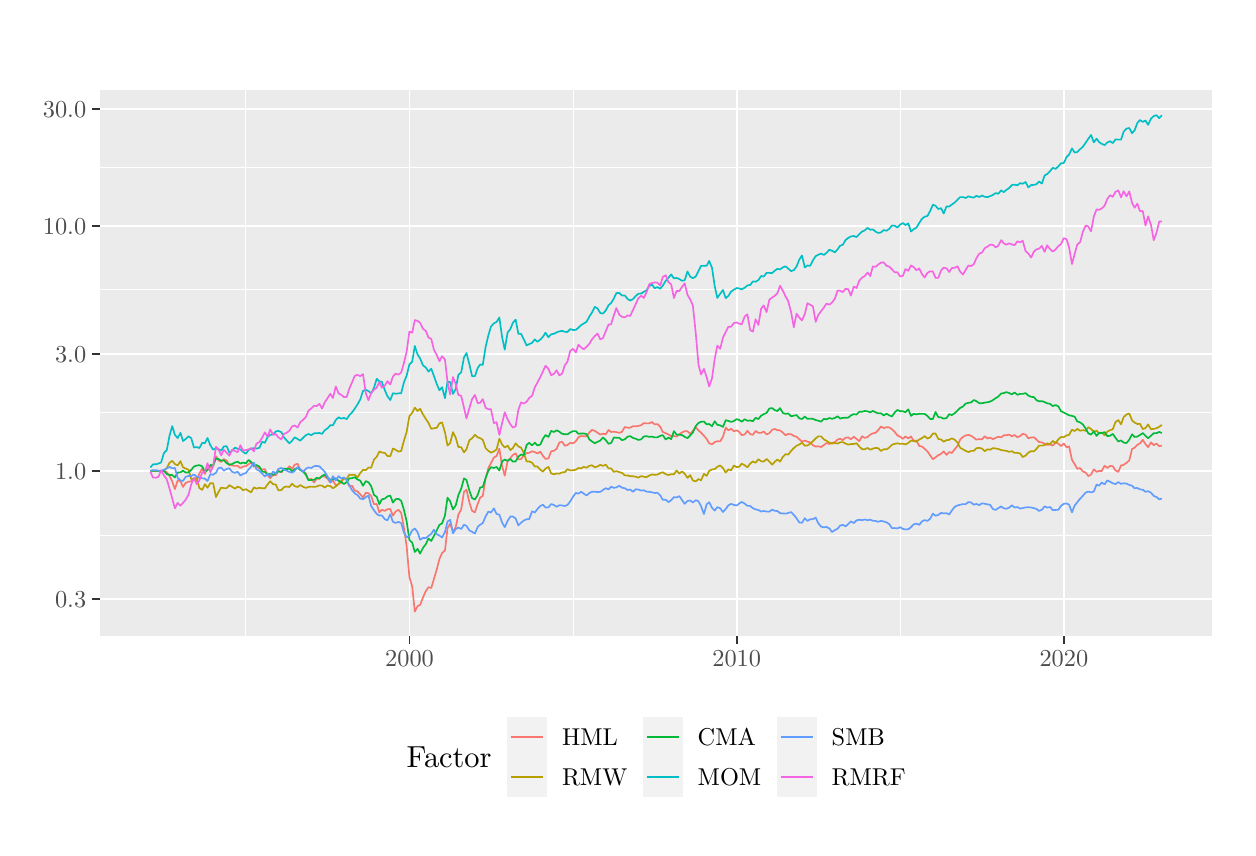
\begin{tikzpicture}[x=1pt,y=1pt]
\definecolor{fillColor}{RGB}{255,255,255}
\path[use as bounding box,fill=fillColor,fill opacity=0.00] (0,0) rectangle (433.62,289.08);
\begin{scope}
\path[clip] (  0.00,  0.00) rectangle (433.62,289.08);
\definecolor{drawColor}{RGB}{255,255,255}
\definecolor{fillColor}{RGB}{255,255,255}

\path[draw=drawColor,line width= 0.6pt,line join=round,line cap=round,fill=fillColor] (  0.00,  0.00) rectangle (433.62,289.08);
\end{scope}
\begin{scope}
\path[clip] ( 26.09, 69.13) rectangle (428.12,266.42);
\definecolor{fillColor}{gray}{0.92}

\path[fill=fillColor] ( 26.09, 69.13) rectangle (428.12,266.42);
\definecolor{drawColor}{RGB}{255,255,255}

\path[draw=drawColor,line width= 0.3pt,line join=round] ( 26.09,105.77) --
	(428.12,105.77);

\path[draw=drawColor,line width= 0.3pt,line join=round] ( 26.09,150.06) --
	(428.12,150.06);

\path[draw=drawColor,line width= 0.3pt,line join=round] ( 26.09,194.35) --
	(428.12,194.35);

\path[draw=drawColor,line width= 0.3pt,line join=round] ( 26.09,238.64) --
	(428.12,238.64);

\path[draw=drawColor,line width= 0.3pt,line join=round] ( 78.85, 69.13) --
	( 78.85,266.42);

\path[draw=drawColor,line width= 0.3pt,line join=round] (197.10, 69.13) --
	(197.10,266.42);

\path[draw=drawColor,line width= 0.3pt,line join=round] (315.33, 69.13) --
	(315.33,266.42);

\path[draw=drawColor,line width= 0.6pt,line join=round] ( 26.09, 82.61) --
	(428.12, 82.61);

\path[draw=drawColor,line width= 0.6pt,line join=round] ( 26.09,128.93) --
	(428.12,128.93);

\path[draw=drawColor,line width= 0.6pt,line join=round] ( 26.09,171.19) --
	(428.12,171.19);

\path[draw=drawColor,line width= 0.6pt,line join=round] ( 26.09,217.51) --
	(428.12,217.51);

\path[draw=drawColor,line width= 0.6pt,line join=round] ( 26.09,259.78) --
	(428.12,259.78);

\path[draw=drawColor,line width= 0.6pt,line join=round] (137.98, 69.13) --
	(137.98,266.42);

\path[draw=drawColor,line width= 0.6pt,line join=round] (256.22, 69.13) --
	(256.22,266.42);

\path[draw=drawColor,line width= 0.6pt,line join=round] (374.43, 69.13) --
	(374.43,266.42);
\definecolor{drawColor}{RGB}{248,118,109}

\path[draw=drawColor,line width= 0.6pt,line join=round] ( 44.36,128.93) --
	( 45.27,128.93) --
	( 46.31,128.93) --
	( 47.28,128.93) --
	( 48.22,128.93) --
	( 49.25,128.93) --
	( 50.26,128.46) --
	( 51.26,127.09) --
	( 52.23,125.08) --
	( 53.20,122.33) --
	( 54.21,125.52) --
	( 55.21,125.16) --
	( 56.15,123.12) --
	( 57.05,124.54) --
	( 58.12,125.01) --
	( 59.09,125.17) --
	( 60.10,126.01) --
	( 61.07,125.20) --
	( 62.04,127.96) --
	( 63.07,129.77) --
	( 64.05,127.77) --
	( 64.98,131.17) --
	( 66.02,130.12) --
	( 67.02,130.66) --
	( 68.03,134.25) --
	( 68.93,132.70) --
	( 69.94,132.19) --
	( 70.88,133.19) --
	( 71.91,132.62) --
	( 72.88,130.99) --
	( 73.82,130.91) --
	( 74.89,130.72) --
	( 75.86,130.72) --
	( 76.86,129.99) --
	( 77.83,130.47) --
	( 78.81,130.66) --
	( 79.84,131.32) --
	( 80.75,131.96) --
	( 81.75,130.45) --
	( 82.66,130.49) --
	( 83.73,129.85) --
	( 84.70,129.36) --
	( 85.70,129.59) --
	( 86.70,127.32) --
	( 87.64,126.29) --
	( 88.68,127.47) --
	( 89.65,127.34) --
	( 90.59,128.98) --
	( 91.66,128.41) --
	( 92.59,129.40) --
	( 93.53,129.44) --
	( 94.57,130.60) --
	( 95.57,129.69) --
	( 96.48,131.16) --
	( 97.55,131.47) --
	( 98.52,129.22) --
	( 99.52,128.93) --
	(100.53,127.99) --
	(101.46,125.66) --
	(102.50,126.09) --
	(103.50,124.71) --
	(104.41,126.06) --
	(105.41,126.05) --
	(106.38,126.96) --
	(107.36,126.89) --
	(108.36,126.11) --
	(109.36,124.68) --
	(110.30,125.42) --
	(111.34,123.69) --
	(112.34,124.18) --
	(113.25,124.66) --
	(114.31,126.48) --
	(115.29,125.60) --
	(116.19,123.45) --
	(117.23,123.55) --
	(118.20,121.74) --
	(119.14,121.57) --
	(120.17,120.47) --
	(121.18,119.32) --
	(122.18,121.00) --
	(123.15,120.85) --
	(124.12,119.81) --
	(125.13,116.88) --
	(126.13,116.96) --
	(127.07,113.92) --
	(127.97,114.87) --
	(129.04,114.45) --
	(130.01,115.11) --
	(131.02,115.13) --
	(131.99,112.73) --
	(132.96,114.27) --
	(134.00,114.89) --
	(134.97,113.71) --
	(135.90,108.72) --
	(136.94,101.67) --
	(137.94, 90.52) --
	(138.95, 87.15) --
	(139.89, 78.10) --
	(140.89, 80.09) --
	(141.80, 80.47) --
	(142.86, 83.21) --
	(143.84, 85.44) --
	(144.84, 86.89) --
	(145.84, 86.62) --
	(146.78, 89.77) --
	(147.82, 93.33) --
	(148.79, 97.08) --
	(149.73, 99.22) --
	(150.79,100.18) --
	(151.70,108.21) --
	(152.67,109.85) --
	(153.68,106.87) --
	(154.68,108.59) --
	(155.62,113.10) --
	(156.65,114.98) --
	(157.66,121.33) --
	(158.56,122.15) --
	(159.63,117.49) --
	(160.60,114.44) --
	(161.61,113.95) --
	(162.61,116.96) --
	(163.52,119.29) --
	(164.45,119.87) --
	(165.49,126.29) --
	(166.49,130.02) --
	(167.40,131.71) --
	(168.47,133.74) --
	(169.44,134.31) --
	(170.44,136.93) --
	(171.45,130.56) --
	(172.39,127.19) --
	(173.42,132.46) --
	(174.42,133.55) --
	(175.33,134.69) --
	(176.33,135.27) --
	(177.31,133.14) --
	(178.28,133.18) --
	(179.28,134.60) --
	(180.28,135.34) --
	(181.22,135.46) --
	(182.26,136.01) --
	(183.26,135.68) --
	(184.17,135.21) --
	(185.24,135.87) --
	(186.21,134.34) --
	(187.11,133.25) --
	(188.18,133.42) --
	(189.15,135.98) --
	(190.16,136.20) --
	(191.13,136.89) --
	(192.10,139.18) --
	(193.13,139.41) --
	(194.10,138.01) --
	(195.04,138.26) --
	(196.08,139.08) --
	(197.08,138.85) --
	(198.09,139.68) --
	(198.99,141.04) --
	(200.00,141.55) --
	(200.93,141.42) --
	(201.97,141.44) --
	(202.94,142.77) --
	(203.88,143.72) --
	(204.95,143.40) --
	(205.92,142.70) --
	(206.92,142.04) --
	(207.89,142.36) --
	(208.87,142.15) --
	(209.90,143.69) --
	(210.81,142.98) --
	(211.81,143.09) --
	(212.72,142.94) --
	(213.79,142.68) --
	(214.76,143.05) --
	(215.76,144.78) --
	(216.76,144.54) --
	(217.70,144.53) --
	(218.74,145.08) --
	(219.71,145.01) --
	(220.65,145.17) --
	(221.72,145.46) --
	(222.62,146.18) --
	(223.59,146.09) --
	(224.60,146.11) --
	(225.60,146.59) --
	(226.54,145.76) --
	(227.57,145.84) --
	(228.58,144.84) --
	(229.48,143.01) --
	(230.55,142.54) --
	(231.52,142.10) --
	(232.53,141.49) --
	(233.53,141.56) --
	(234.47,141.31) --
	(235.47,142.18) --
	(236.44,142.82) --
	(237.41,143.28) --
	(238.42,143.27) --
	(239.42,142.22) --
	(240.36,143.41) --
	(241.40,144.71) --
	(242.40,143.55) --
	(243.31,142.76) --
	(244.37,141.61) --
	(245.35,140.46) --
	(246.25,138.93) --
	(247.29,138.53) --
	(248.26,139.32) --
	(249.20,139.65) --
	(250.23,139.56) --
	(251.24,141.29) --
	(252.24,144.58) --
	(253.21,143.58) --
	(254.18,144.14) --
	(255.19,143.23) --
	(256.19,143.60) --
	(257.13,142.98) --
	(258.03,141.83) --
	(259.10,142.09) --
	(260.07,143.41) --
	(261.08,142.23) --
	(262.05,141.97) --
	(263.02,143.34) --
	(264.05,142.68) --
	(265.03,142.65) --
	(265.96,143.14) --
	(267.00,142.13) --
	(268.00,142.54) --
	(269.01,143.76) --
	(269.91,144.07) --
	(270.92,143.63) --
	(271.86,143.55) --
	(272.89,142.74) --
	(273.86,141.83) --
	(274.80,142.25) --
	(275.87,142.17) --
	(276.84,141.55) --
	(277.84,141.25) --
	(278.82,140.37) --
	(279.79,139.49) --
	(280.82,139.87) --
	(281.76,139.52) --
	(282.73,139.20) --
	(283.74,138.20) --
	(284.74,137.69) --
	(285.68,137.83) --
	(286.71,137.54) --
	(287.72,138.25) --
	(288.62,138.96) --
	(289.69,138.65) --
	(290.66,139.03) --
	(291.67,139.34) --
	(292.67,140.26) --
	(293.58,140.54) --
	(294.51,140.05) --
	(295.55,140.89) --
	(296.55,141.01) --
	(297.46,140.36) --
	(298.53,141.26) --
	(299.50,140.46) --
	(300.50,139.67) --
	(301.51,141.44) --
	(302.44,140.83) --
	(303.48,141.14) --
	(304.48,142.06) --
	(305.39,142.49) --
	(306.39,142.69) --
	(307.36,143.67) --
	(308.34,144.95) --
	(309.34,144.40) --
	(310.34,144.70) --
	(311.28,144.65) --
	(312.32,143.99) --
	(313.32,142.98) --
	(314.23,141.78) --
	(315.30,141.25) --
	(316.27,140.50) --
	(317.17,141.36) --
	(318.21,140.68) --
	(319.18,141.36) --
	(320.12,139.85) --
	(321.15,139.88) --
	(322.16,137.93) --
	(323.16,137.73) --
	(324.13,136.89) --
	(325.10,136.00) --
	(326.11,134.53) --
	(327.11,133.16) --
	(328.05,133.81) --
	(329.05,134.60) --
	(330.06,135.08) --
	(330.99,135.94) --
	(332.03,134.71) --
	(333.00,135.75) --
	(333.94,135.39) --
	(335.01,136.77) --
	(335.98,138.02) --
	(336.98,140.28) --
	(337.95,141.16) --
	(338.92,141.74) --
	(339.96,141.90) --
	(340.87,141.64) --
	(341.87,140.97) --
	(342.78,140.22) --
	(343.85,140.42) --
	(344.82,140.30) --
	(345.82,141.43) --
	(346.82,140.63) --
	(347.76,140.93) --
	(348.80,140.41) --
	(349.77,140.86) --
	(350.71,141.25) --
	(351.78,141.02) --
	(352.68,141.78) --
	(353.65,141.80) --
	(354.66,142.05) --
	(355.66,141.41) --
	(356.60,141.89) --
	(357.63,141.11) --
	(358.64,141.51) --
	(359.54,142.31) --
	(360.61,142.03) --
	(361.58,140.70) --
	(362.59,140.99) --
	(363.59,141.06) --
	(364.50,140.27) --
	(365.44,139.37) --
	(366.47,139.24) --
	(367.47,138.75) --
	(368.38,138.33) --
	(369.45,138.45) --
	(370.42,138.06) --
	(371.42,139.21) --
	(372.43,138.76) --
	(373.37,137.90) --
	(374.40,138.80) --
	(375.41,137.44) --
	(376.31,137.79) --
	(377.35,132.93) --
	(378.32,131.35) --
	(379.26,129.67) --
	(380.29,129.95) --
	(381.30,128.69) --
	(382.30,128.32) --
	(383.27,127.04) --
	(384.24,127.58) --
	(385.25,129.49) --
	(386.25,128.58) --
	(387.19,128.93) --
	(388.09,128.87) --
	(389.16,130.81) --
	(390.13,129.99) --
	(391.14,130.70) --
	(392.11,130.60) --
	(393.08,129.08) --
	(394.11,128.61) --
	(395.09,130.90) --
	(396.02,131.10) --
	(397.06,131.83) --
	(398.06,132.70) --
	(399.07,136.88) --
	(399.97,137.26) --
	(400.98,138.34) --
	(401.92,138.85) --
	(402.95,140.16) --
	(403.92,138.63) --
	(404.86,137.49) --
	(405.93,139.21) --
	(406.90,138.21) --
	(407.90,138.79) --
	(408.87,137.87) --
	(409.85,138.06);
\definecolor{drawColor}{RGB}{183,159,0}

\path[draw=drawColor,line width= 0.6pt,line join=round] ( 44.36,128.93) --
	( 45.27,128.93) --
	( 46.31,128.93) --
	( 47.28,128.93) --
	( 48.22,128.93) --
	( 49.25,128.93) --
	( 50.26,130.00) --
	( 51.26,131.84) --
	( 52.23,132.55) --
	( 53.20,131.40) --
	( 54.21,130.90) --
	( 55.21,132.46) --
	( 56.15,130.16) --
	( 57.05,129.81) --
	( 58.12,129.34) --
	( 59.09,125.96) --
	( 60.10,126.06) --
	( 61.07,126.43) --
	( 62.04,122.70) --
	( 63.07,122.06) --
	( 64.05,124.12) --
	( 64.98,122.84) --
	( 66.02,124.49) --
	( 67.02,124.46) --
	( 68.03,119.44) --
	( 68.93,121.23) --
	( 69.94,122.89) --
	( 70.88,122.71) --
	( 71.91,122.68) --
	( 72.88,123.76) --
	( 73.82,123.18) --
	( 74.89,122.52) --
	( 75.86,123.20) --
	( 76.86,122.86) --
	( 77.83,121.95) --
	( 78.81,122.32) --
	( 79.84,121.69) --
	( 80.75,121.18) --
	( 81.75,122.97) --
	( 82.66,122.51) --
	( 83.73,122.82) --
	( 84.70,122.64) --
	( 85.70,122.63) --
	( 86.70,124.04) --
	( 87.64,125.18) --
	( 88.68,124.10) --
	( 89.65,124.00) --
	( 90.59,121.90) --
	( 91.66,121.98) --
	( 92.59,123.01) --
	( 93.53,123.27) --
	( 94.57,123.11) --
	( 95.57,124.27) --
	( 96.48,123.40) --
	( 97.55,123.10) --
	( 98.52,123.82) --
	( 99.52,123.16) --
	(100.53,122.77) --
	(101.46,123.12) --
	(102.50,123.24) --
	(103.50,123.13) --
	(104.41,123.28) --
	(105.41,123.69) --
	(106.38,123.59) --
	(107.36,122.89) --
	(108.36,123.64) --
	(109.36,123.42) --
	(110.30,122.67) --
	(111.34,123.28) --
	(112.34,124.22) --
	(113.25,125.29) --
	(114.31,126.16) --
	(115.29,126.10) --
	(116.19,127.51) --
	(117.23,127.46) --
	(118.20,127.52) --
	(119.14,126.48) --
	(120.17,128.14) --
	(121.18,129.32) --
	(122.18,129.17) --
	(123.15,130.13) --
	(124.12,130.07) --
	(125.13,133.01) --
	(126.13,134.05) --
	(127.07,135.93) --
	(127.97,135.56) --
	(129.04,135.41) --
	(130.01,134.29) --
	(131.02,134.23) --
	(131.99,137.01) --
	(132.96,136.52) --
	(134.00,135.92) --
	(134.97,136.13) --
	(135.90,139.65) --
	(136.94,142.99) --
	(137.94,148.72) --
	(138.95,149.91) --
	(139.89,151.78) --
	(140.89,150.58) --
	(141.80,151.36) --
	(142.86,149.32) --
	(143.84,147.73) --
	(144.84,146.23) --
	(145.84,144.10) --
	(146.78,144.34) --
	(147.82,144.49) --
	(148.79,146.11) --
	(149.73,146.42) --
	(150.79,142.86) --
	(151.70,138.09) --
	(152.67,138.94) --
	(153.68,142.95) --
	(154.68,140.87) --
	(155.62,137.58) --
	(156.65,137.48) --
	(157.66,135.60) --
	(158.56,136.75) --
	(159.63,140.07) --
	(160.60,140.69) --
	(161.61,141.97) --
	(162.61,141.05) --
	(163.52,140.75) --
	(164.45,140.17) --
	(165.49,137.12) --
	(166.49,136.15) --
	(167.40,135.52) --
	(168.47,135.98) --
	(169.44,136.67) --
	(170.44,140.55) --
	(171.45,138.46) --
	(172.39,137.35) --
	(173.42,138.05) --
	(174.42,136.41) --
	(175.33,137.20) --
	(176.33,138.89) --
	(177.31,137.74) --
	(178.28,137.32) --
	(179.28,135.44) --
	(180.28,132.34) --
	(181.22,132.34) --
	(182.26,131.88) --
	(183.26,130.48) --
	(184.17,130.51) --
	(185.24,129.35) --
	(186.21,128.64) --
	(187.11,129.76) --
	(188.18,130.37) --
	(189.15,128.03) --
	(190.16,127.69) --
	(191.13,127.97) --
	(192.10,127.91) --
	(193.13,128.39) --
	(194.10,128.45) --
	(195.04,129.53) --
	(196.08,129.08) --
	(197.08,129.16) --
	(198.09,129.33) --
	(198.99,129.95) --
	(200.00,129.85) --
	(200.93,130.37) --
	(201.97,130.07) --
	(202.94,130.74) --
	(203.88,130.96) --
	(204.95,130.22) --
	(205.92,130.55) --
	(206.92,131.12) --
	(207.89,130.71) --
	(208.87,131.20) --
	(209.90,129.82) --
	(210.81,129.85) --
	(211.81,128.55) --
	(212.72,128.86) --
	(213.79,128.49) --
	(214.76,128.20) --
	(215.76,127.31) --
	(216.76,127.26) --
	(217.70,127.03) --
	(218.74,126.97) --
	(219.71,126.81) --
	(220.65,126.48) --
	(221.72,127.02) --
	(222.62,126.81) --
	(223.59,126.64) --
	(224.60,127.23) --
	(225.60,127.64) --
	(226.54,127.49) --
	(227.57,127.60) --
	(228.58,128.14) --
	(229.48,128.43) --
	(230.55,127.75) --
	(231.52,127.43) --
	(232.53,127.72) --
	(233.53,127.71) --
	(234.47,129.07) --
	(235.47,127.94) --
	(236.44,128.73) --
	(237.41,127.91) --
	(238.42,126.41) --
	(239.42,127.38) --
	(240.36,125.47) --
	(241.40,125.11) --
	(242.40,125.96) --
	(243.31,125.52) --
	(244.37,127.84) --
	(245.35,127.12) --
	(246.25,128.90) --
	(247.29,129.46) --
	(248.26,129.58) --
	(249.20,130.40) --
	(250.23,130.90) --
	(251.24,129.94) --
	(252.24,128.29) --
	(253.21,129.49) --
	(254.18,129.09) --
	(255.19,130.85) --
	(256.19,130.27) --
	(257.13,130.43) --
	(258.03,131.55) --
	(259.10,130.95) --
	(260.07,130.22) --
	(261.08,131.56) --
	(262.05,132.35) --
	(263.02,131.86) --
	(264.05,133.16) --
	(265.03,132.38) --
	(265.96,132.28) --
	(267.00,133.23) --
	(268.00,132.30) --
	(269.01,131.17) --
	(269.91,132.17) --
	(270.92,133.05) --
	(271.86,132.26) --
	(272.89,133.98) --
	(273.86,134.98) --
	(274.80,134.79) --
	(275.87,136.14) --
	(276.84,137.18) --
	(277.84,138.01) --
	(278.82,138.44) --
	(279.79,139.13) --
	(280.82,138.02) --
	(281.76,138.10) --
	(282.73,138.70) --
	(283.74,139.64) --
	(284.74,140.66) --
	(285.68,141.41) --
	(286.71,141.39) --
	(287.72,140.28) --
	(288.62,139.81) --
	(289.69,139.14) --
	(290.66,138.79) --
	(291.67,138.99) --
	(292.67,138.79) --
	(293.58,139.27) --
	(294.51,139.33) --
	(295.55,138.80) --
	(296.55,138.39) --
	(297.46,138.61) --
	(298.53,138.65) --
	(299.50,138.92) --
	(300.50,137.72) --
	(301.51,136.77) --
	(302.44,136.74) --
	(303.48,137.20) --
	(304.48,136.57) --
	(305.39,136.97) --
	(306.39,137.22) --
	(307.36,137.13) --
	(308.34,136.13) --
	(309.34,136.76) --
	(310.34,136.70) --
	(311.28,137.31) --
	(312.32,138.39) --
	(313.32,138.69) --
	(314.23,138.89) --
	(315.30,138.67) --
	(316.27,138.73) --
	(317.17,138.49) --
	(318.21,139.04) --
	(319.18,139.86) --
	(320.12,139.69) --
	(321.15,139.51) --
	(322.16,140.24) --
	(323.16,140.78) --
	(324.13,141.49) --
	(325.10,140.61) --
	(326.11,141.04) --
	(327.11,142.42) --
	(328.05,142.43) --
	(329.05,140.47) --
	(330.06,140.27) --
	(330.99,139.47) --
	(332.03,140.04) --
	(333.00,140.14) --
	(333.94,140.71) --
	(335.01,140.16) --
	(335.98,139.17) --
	(336.98,137.25) --
	(337.95,136.72) --
	(338.92,136.17) --
	(339.96,135.70) --
	(340.87,136.16) --
	(341.87,136.14) --
	(342.78,137.10) --
	(343.85,137.26) --
	(344.82,136.99) --
	(345.82,136.04) --
	(346.82,136.73) --
	(347.76,136.56) --
	(348.80,137.17) --
	(349.77,137.01) --
	(350.71,136.86) --
	(351.78,136.44) --
	(352.68,136.29) --
	(353.65,136.17) --
	(354.66,135.79) --
	(355.66,136.04) --
	(356.60,135.42) --
	(357.63,135.42) --
	(358.64,135.21) --
	(359.54,133.93) --
	(360.61,134.46) --
	(361.58,135.52) --
	(362.59,136.05) --
	(363.59,135.97) --
	(364.50,136.85) --
	(365.44,138.06) --
	(366.47,138.06) --
	(367.47,138.23) --
	(368.38,138.87) --
	(369.45,138.61) --
	(370.42,139.77) --
	(371.42,138.97) --
	(372.43,140.34) --
	(373.37,141.17) --
	(374.40,141.09) --
	(375.41,141.77) --
	(376.31,141.94) --
	(377.35,143.81) --
	(378.32,143.32) --
	(379.26,144.09) --
	(380.29,143.42) --
	(381.30,143.66) --
	(382.30,143.38) --
	(383.27,144.75) --
	(384.24,144.06) --
	(385.25,143.12) --
	(386.25,143.45) --
	(387.19,142.48) --
	(388.09,142.78) --
	(389.16,141.80) --
	(390.13,143.15) --
	(391.14,143.63) --
	(392.11,144.00) --
	(393.08,146.57) --
	(394.11,147.28) --
	(395.09,145.73) --
	(396.02,148.35) --
	(397.06,149.29) --
	(398.06,149.68) --
	(399.07,147.16) --
	(399.97,146.39) --
	(400.98,145.86) --
	(401.92,145.93) --
	(402.95,144.03) --
	(403.92,144.40) --
	(404.86,145.70) --
	(405.93,143.95) --
	(406.90,144.12) --
	(407.90,144.32) --
	(408.87,144.86) --
	(409.85,145.54);
\definecolor{drawColor}{RGB}{0,186,56}

\path[draw=drawColor,line width= 0.6pt,line join=round] ( 44.36,128.93) --
	( 45.27,128.93) --
	( 46.31,128.93) --
	( 47.28,128.93) --
	( 48.22,128.93) --
	( 49.25,128.93) --
	( 50.26,127.73) --
	( 51.26,127.46) --
	( 52.23,127.41) --
	( 53.20,126.57) --
	( 54.21,128.32) --
	( 55.21,128.41) --
	( 56.15,128.99) --
	( 57.05,128.35) --
	( 58.12,128.37) --
	( 59.09,129.25) --
	( 60.10,130.51) --
	( 61.07,130.84) --
	( 62.04,131.01) --
	( 63.07,130.55) --
	( 64.05,128.58) --
	( 64.98,129.15) --
	( 66.02,131.07) --
	( 67.02,130.86) --
	( 68.03,133.41) --
	( 68.93,133.20) --
	( 69.94,132.63) --
	( 70.88,132.76) --
	( 71.91,131.69) --
	( 72.88,131.21) --
	( 73.82,131.37) --
	( 74.89,131.95) --
	( 75.86,132.23) --
	( 76.86,131.58) --
	( 77.83,131.93) --
	( 78.81,131.63) --
	( 79.84,132.87) --
	( 80.75,132.12) --
	( 81.75,130.79) --
	( 82.66,131.04) --
	( 83.73,130.50) --
	( 84.70,128.73) --
	( 85.70,128.52) --
	( 86.70,127.73) --
	( 87.64,127.79) --
	( 88.68,127.48) --
	( 89.65,128.09) --
	( 90.59,128.71) --
	( 91.66,128.55) --
	( 92.59,129.78) --
	( 93.53,129.56) --
	( 94.57,129.73) --
	( 95.57,128.79) --
	( 96.48,129.57) --
	( 97.55,130.08) --
	( 98.52,129.20) --
	( 99.52,128.69) --
	(100.53,127.49) --
	(101.46,125.58) --
	(102.50,125.65) --
	(103.50,125.68) --
	(104.41,126.38) --
	(105.41,126.21) --
	(106.38,127.08) --
	(107.36,127.65) --
	(108.36,126.55) --
	(109.36,125.70) --
	(110.30,125.79) --
	(111.34,126.26) --
	(112.34,125.33) --
	(113.25,124.91) --
	(114.31,124.17) --
	(115.29,124.91) --
	(116.19,126.19) --
	(117.23,126.30) --
	(118.20,126.63) --
	(119.14,125.82) --
	(120.17,125.43) --
	(121.18,123.54) --
	(122.18,125.23) --
	(123.15,124.80) --
	(124.12,123.42) --
	(125.13,120.25) --
	(126.13,119.54) --
	(127.07,116.89) --
	(127.97,118.60) --
	(129.04,118.91) --
	(130.01,119.69) --
	(131.02,120.01) --
	(131.99,117.44) --
	(132.96,118.70) --
	(134.00,118.83) --
	(134.97,118.09) --
	(135.90,115.05) --
	(136.94,110.67) --
	(137.94,103.94) --
	(138.95,103.01) --
	(139.89, 99.61) --
	(140.89,100.75) --
	(141.80, 99.02) --
	(142.86,101.12) --
	(143.84,102.42) --
	(144.84,104.47) --
	(145.84,103.60) --
	(146.78,105.42) --
	(147.82,107.43) --
	(148.79,109.42) --
	(149.73,109.95) --
	(150.79,112.80) --
	(151.70,119.26) --
	(152.67,117.93) --
	(153.68,114.99) --
	(154.68,116.46) --
	(155.62,120.15) --
	(156.65,122.46) --
	(157.66,126.20) --
	(158.56,125.64) --
	(159.63,121.69) --
	(160.60,119.04) --
	(161.61,118.57) --
	(162.61,120.20) --
	(163.52,122.93) --
	(164.45,123.12) --
	(165.49,126.40) --
	(166.49,129.03) --
	(167.40,130.26) --
	(168.47,129.98) --
	(169.44,130.35) --
	(170.44,129.05) --
	(171.45,132.34) --
	(172.39,133.02) --
	(173.42,132.55) --
	(174.42,133.23) --
	(175.33,132.27) --
	(176.33,132.34) --
	(177.31,134.07) --
	(178.28,134.84) --
	(179.28,134.62) --
	(180.28,138.26) --
	(181.22,139.07) --
	(182.26,138.14) --
	(183.26,139.13) --
	(184.17,138.13) --
	(185.24,138.42) --
	(186.21,140.55) --
	(187.11,141.87) --
	(188.18,141.20) --
	(189.15,143.38) --
	(190.16,142.97) --
	(191.13,143.58) --
	(192.10,143.10) --
	(193.13,142.31) --
	(194.10,142.19) --
	(195.04,142.10) --
	(196.08,142.82) --
	(197.08,143.29) --
	(198.09,143.29) --
	(198.99,142.30) --
	(200.00,142.46) --
	(200.93,142.46) --
	(201.97,142.20) --
	(202.94,140.31) --
	(203.88,139.58) --
	(204.95,138.90) --
	(205.92,139.41) --
	(206.92,139.88) --
	(207.89,141.01) --
	(208.87,140.06) --
	(209.90,138.71) --
	(210.81,138.99) --
	(211.81,141.00) --
	(212.72,140.89) --
	(213.79,140.85) --
	(214.76,140.02) --
	(215.76,140.32) --
	(216.76,141.28) --
	(217.70,141.49) --
	(218.74,140.84) --
	(219.71,140.55) --
	(220.65,140.10) --
	(221.72,140.34) --
	(222.62,141.33) --
	(223.59,141.48) --
	(224.60,141.20) --
	(225.60,141.33) --
	(226.54,141.02) --
	(227.57,141.05) --
	(228.58,141.60) --
	(229.48,141.84) --
	(230.55,140.28) --
	(231.52,140.96) --
	(232.53,140.40) --
	(233.53,143.31) --
	(234.47,142.03) --
	(235.47,141.99) --
	(236.44,141.87) --
	(237.41,141.22) --
	(238.42,140.77) --
	(239.42,141.74) --
	(240.36,142.78) --
	(241.40,145.12) --
	(242.40,146.24) --
	(243.31,146.68) --
	(244.37,146.74) --
	(245.35,145.77) --
	(246.25,145.86) --
	(247.29,145.06) --
	(248.26,146.86) --
	(249.20,145.58) --
	(250.23,145.38) --
	(251.24,144.80) --
	(252.24,147.25) --
	(253.21,146.98) --
	(254.18,146.63) --
	(255.19,146.92) --
	(256.19,147.63) --
	(257.13,147.31) --
	(258.03,146.68) --
	(259.10,147.60) --
	(260.07,147.03) --
	(261.08,147.16) --
	(262.05,146.86) --
	(263.02,148.09) --
	(264.05,147.65) --
	(265.03,148.86) --
	(265.96,149.43) --
	(267.00,149.87) --
	(268.00,151.46) --
	(269.01,151.62) --
	(269.91,150.90) --
	(270.92,150.55) --
	(271.86,151.61) --
	(272.89,149.87) --
	(273.86,149.51) --
	(274.80,149.71) --
	(275.87,148.66) --
	(276.84,148.87) --
	(277.84,149.10) --
	(278.82,147.94) --
	(279.79,147.65) --
	(280.82,148.54) --
	(281.76,147.71) --
	(282.73,147.82) --
	(283.74,147.73) --
	(284.74,147.28) --
	(285.68,147.08) --
	(286.71,146.72) --
	(287.72,147.73) --
	(288.62,147.51) --
	(289.69,148.03) --
	(290.66,147.74) --
	(291.67,148.05) --
	(292.67,148.65) --
	(293.58,147.83) --
	(294.51,148.09) --
	(295.55,148.11) --
	(296.55,148.17) --
	(297.46,148.96) --
	(298.53,149.43) --
	(299.50,149.27) --
	(300.50,150.32) --
	(301.51,150.27) --
	(302.44,150.57) --
	(303.48,150.43) --
	(304.48,150.08) --
	(305.39,150.60) --
	(306.39,150.08) --
	(307.36,149.70) --
	(308.34,149.75) --
	(309.34,148.95) --
	(310.34,149.60) --
	(311.28,149.02) --
	(312.32,148.59) --
	(313.32,150.06) --
	(314.23,150.94) --
	(315.30,150.48) --
	(316.27,150.46) --
	(317.17,150.11) --
	(318.21,151.16) --
	(319.18,148.78) --
	(320.12,149.54) --
	(321.15,149.35) --
	(322.16,149.57) --
	(323.16,149.51) --
	(324.13,149.51) --
	(325.10,148.80) --
	(326.11,147.68) --
	(327.11,147.69) --
	(328.05,150.20) --
	(329.05,148.34) --
	(330.06,148.25) --
	(330.99,147.79) --
	(332.03,148.01) --
	(333.00,149.43) --
	(333.94,149.08) --
	(335.01,149.81) --
	(335.98,150.73) --
	(336.98,151.69) --
	(337.95,152.17) --
	(338.92,153.21) --
	(339.96,153.55) --
	(340.87,153.62) --
	(341.87,154.54) --
	(342.78,154.13) --
	(343.85,153.38) --
	(344.82,153.36) --
	(345.82,153.59) --
	(346.82,153.72) --
	(347.76,153.96) --
	(348.80,154.51) --
	(349.77,155.19) --
	(350.71,155.78) --
	(351.78,156.88) --
	(352.68,157.03) --
	(353.65,157.38) --
	(354.66,157.03) --
	(355.66,156.57) --
	(356.60,157.27) --
	(357.63,156.43) --
	(358.64,156.76) --
	(359.54,156.75) --
	(360.61,157.02) --
	(361.58,156.12) --
	(362.59,155.70) --
	(363.59,155.58) --
	(364.50,154.51) --
	(365.44,154.05) --
	(366.47,154.13) --
	(367.47,153.81) --
	(368.38,153.34) --
	(369.45,153.15) --
	(370.42,152.34) --
	(371.42,152.72) --
	(372.43,152.25) --
	(373.37,150.51) --
	(374.40,149.99) --
	(375.41,149.49) --
	(376.31,149.01) --
	(377.35,148.80) --
	(378.32,148.50) --
	(379.26,146.80) --
	(380.29,146.47) --
	(381.30,145.70) --
	(382.30,144.21) --
	(383.27,142.46) --
	(384.24,142.04) --
	(385.25,143.19) --
	(386.25,141.58) --
	(387.19,142.68) --
	(388.09,142.57) --
	(389.16,142.92) --
	(390.13,141.46) --
	(391.14,141.62) --
	(392.11,142.29) --
	(393.08,140.89) --
	(394.11,139.54) --
	(395.09,139.93) --
	(396.02,139.15) --
	(397.06,138.98) --
	(398.06,140.19) --
	(399.07,142.16) --
	(399.97,141.18) --
	(400.98,141.31) --
	(401.92,141.88) --
	(402.95,142.58) --
	(403.92,141.59) --
	(404.86,140.74) --
	(405.93,141.64) --
	(406.90,142.55) --
	(407.90,142.56) --
	(408.87,142.99) --
	(409.85,142.62);
\definecolor{drawColor}{RGB}{0,191,196}

\path[draw=drawColor,line width= 0.6pt,line join=round] ( 44.36,130.15) --
	( 45.27,131.29) --
	( 46.31,131.30) --
	( 47.28,131.58) --
	( 48.22,131.97) --
	( 49.25,135.40) --
	( 50.26,136.42) --
	( 51.26,141.66) --
	( 52.23,145.09) --
	( 53.20,141.96) --
	( 54.21,140.78) --
	( 55.21,142.67) --
	( 56.15,139.71) --
	( 57.05,140.41) --
	( 58.12,141.40) --
	( 59.09,140.77) --
	( 60.10,137.36) --
	( 61.07,137.53) --
	( 62.04,137.16) --
	( 63.07,139.06) --
	( 64.05,138.96) --
	( 64.98,140.81) --
	( 66.02,138.13) --
	( 67.02,136.59) --
	( 68.03,137.09) --
	( 68.93,136.75) --
	( 69.94,136.24) --
	( 70.88,137.74) --
	( 71.91,137.87) --
	( 72.88,135.50) --
	( 73.82,136.17) --
	( 74.89,137.33) --
	( 75.86,136.93) --
	( 76.86,136.68) --
	( 77.83,135.81) --
	( 78.81,135.09) --
	( 79.84,136.48) --
	( 80.75,136.92) --
	( 81.75,137.17) --
	( 82.66,136.98) --
	( 83.73,137.26) --
	( 84.70,139.44) --
	( 85.70,139.06) --
	( 86.70,141.17) --
	( 87.64,141.94) --
	( 88.68,142.09) --
	( 89.65,143.19) --
	( 90.59,143.37) --
	( 91.66,142.92) --
	( 92.59,141.04) --
	( 93.53,139.99) --
	( 94.57,138.86) --
	( 95.57,139.84) --
	( 96.48,141.06) --
	( 97.55,140.44) --
	( 98.52,139.84) --
	( 99.52,140.90) --
	(100.53,141.81) --
	(101.46,142.26) --
	(102.50,141.83) --
	(103.50,142.49) --
	(104.41,142.52) --
	(105.41,142.62) --
	(106.38,142.32) --
	(107.36,143.63) --
	(108.36,144.31) --
	(109.36,145.40) --
	(110.30,145.38) --
	(111.34,147.32) --
	(112.34,148.29) --
	(113.25,147.82) --
	(114.31,148.06) --
	(115.29,147.63) --
	(116.19,149.00) --
	(117.23,150.09) --
	(118.20,151.42) --
	(119.14,152.88) --
	(120.17,154.72) --
	(121.18,157.82) --
	(122.18,158.24) --
	(123.15,157.75) --
	(124.12,156.93) --
	(125.13,158.95) --
	(126.13,162.20) --
	(127.07,161.24) --
	(127.97,161.11) --
	(129.04,158.12) --
	(130.01,155.90) --
	(131.02,154.51) --
	(131.99,156.98) --
	(132.96,156.80) --
	(134.00,156.94) --
	(134.97,156.97) --
	(135.90,160.74) --
	(136.94,163.38) --
	(137.94,167.39) --
	(138.95,168.38) --
	(139.89,174.04) --
	(140.89,171.00) --
	(141.80,169.55) --
	(142.86,167.04) --
	(143.84,166.30) --
	(144.84,164.79) --
	(145.84,165.85) --
	(146.78,163.27) --
	(147.82,160.35) --
	(148.79,158.05) --
	(149.73,159.16) --
	(150.79,155.20) --
	(151.70,161.14) --
	(152.67,161.00) --
	(153.68,156.73) --
	(154.68,158.49) --
	(155.62,163.65) --
	(156.65,164.52) --
	(157.66,169.91) --
	(158.56,171.51) --
	(159.63,167.35) --
	(160.60,163.13) --
	(161.61,163.18) --
	(162.61,166.09) --
	(163.52,167.38) --
	(164.45,167.21) --
	(165.49,173.80) --
	(166.49,177.99) --
	(167.40,181.04) --
	(168.47,182.26) --
	(169.44,182.73) --
	(170.44,184.34) --
	(171.45,177.15) --
	(172.39,172.73) --
	(173.42,178.92) --
	(174.42,180.17) --
	(175.33,182.50) --
	(176.33,183.58) --
	(177.31,178.45) --
	(178.28,178.42) --
	(179.28,176.48) --
	(180.28,174.26) --
	(181.22,174.71) --
	(182.26,175.19) --
	(183.26,176.44) --
	(184.17,175.56) --
	(185.24,176.38) --
	(186.21,177.39) --
	(187.11,178.85) --
	(188.18,177.23) --
	(189.15,178.29) --
	(190.16,178.45) --
	(191.13,178.98) --
	(192.10,179.33) --
	(193.13,179.52) --
	(194.10,179.19) --
	(195.04,179.11) --
	(196.08,180.19) --
	(197.08,179.82) --
	(198.09,179.90) --
	(198.99,180.64) --
	(200.00,181.61) --
	(200.93,182.17) --
	(201.97,182.81) --
	(202.94,184.65) --
	(203.88,186.11) --
	(204.95,188.20) --
	(205.92,187.60) --
	(206.92,185.97) --
	(207.89,185.77) --
	(208.87,186.85) --
	(209.90,188.82) --
	(210.81,189.54) --
	(211.81,191.22) --
	(212.72,193.17) --
	(213.79,193.20) --
	(214.76,192.29) --
	(215.76,192.34) --
	(216.76,191.07) --
	(217.70,190.47) --
	(218.74,191.01) --
	(219.71,192.10) --
	(220.65,192.94) --
	(221.72,193.02) --
	(222.62,193.61) --
	(223.59,194.17) --
	(224.60,195.70) --
	(225.60,196.26) --
	(226.54,194.92) --
	(227.57,195.34) --
	(228.58,194.75) --
	(229.48,195.84) --
	(230.55,197.61) --
	(231.52,198.69) --
	(232.53,199.90) --
	(233.53,198.47) --
	(234.47,198.66) --
	(235.47,198.25) --
	(236.44,197.63) --
	(237.41,197.81) --
	(238.42,200.97) --
	(239.42,199.08) --
	(240.36,198.56) --
	(241.40,199.14) --
	(242.40,201.18) --
	(243.31,203.01) --
	(244.37,203.02) --
	(245.35,203.03) --
	(246.25,204.81) --
	(247.29,202.27) --
	(248.26,195.66) --
	(249.20,191.43) --
	(250.23,192.92) --
	(251.24,194.31) --
	(252.24,191.35) --
	(253.21,192.15) --
	(254.18,193.71) --
	(255.19,194.39) --
	(256.19,195.00) --
	(257.13,194.84) --
	(258.03,194.54) --
	(259.10,195.11) --
	(260.07,195.93) --
	(261.08,196.10) --
	(262.05,197.38) --
	(263.02,197.28) --
	(264.05,197.87) --
	(265.03,199.35) --
	(265.96,199.12) --
	(267.00,200.49) --
	(268.00,200.46) --
	(269.01,200.42) --
	(269.91,201.22) --
	(270.92,201.95) --
	(271.86,201.71) --
	(272.89,202.47) --
	(273.86,202.85) --
	(274.80,202.03) --
	(275.87,201.11) --
	(276.84,201.46) --
	(277.84,202.78) --
	(278.82,205.27) --
	(279.79,206.76) --
	(280.82,202.43) --
	(281.76,203.14) --
	(282.73,203.01) --
	(283.74,204.98) --
	(284.74,206.52) --
	(285.68,207.02) --
	(286.71,207.46) --
	(287.72,206.93) --
	(288.62,207.71) --
	(289.69,208.83) --
	(290.66,208.46) --
	(291.67,207.90) --
	(292.67,209.00) --
	(293.58,210.29) --
	(294.51,210.59) --
	(295.55,212.34) --
	(296.55,213.14) --
	(297.46,213.63) --
	(298.53,213.80) --
	(299.50,213.40) --
	(300.50,214.48) --
	(301.51,215.40) --
	(302.44,215.79) --
	(303.48,216.72) --
	(304.48,216.05) --
	(305.39,216.21) --
	(306.39,215.38) --
	(307.36,214.90) --
	(308.34,215.09) --
	(309.34,215.94) --
	(310.34,215.70) --
	(311.28,216.33) --
	(312.32,217.59) --
	(313.32,217.51) --
	(314.23,216.85) --
	(315.30,217.93) --
	(316.27,218.49) --
	(317.17,217.75) --
	(318.21,218.34) --
	(319.18,215.41) --
	(320.12,216.23) --
	(321.15,216.81) --
	(322.16,218.52) --
	(323.16,219.99) --
	(324.13,220.80) --
	(325.10,220.99) --
	(326.11,222.85) --
	(327.11,225.09) --
	(328.05,224.73) --
	(329.05,223.54) --
	(330.06,223.87) --
	(330.99,221.93) --
	(332.03,224.51) --
	(333.00,224.44) --
	(333.94,225.16) --
	(335.01,225.91) --
	(335.98,226.91) --
	(336.98,227.86) --
	(337.95,227.86) --
	(338.92,227.53) --
	(339.96,228.15) --
	(340.87,227.83) --
	(341.87,227.66) --
	(342.78,228.33) --
	(343.85,227.89) --
	(344.82,228.42) --
	(345.82,227.98) --
	(346.82,227.84) --
	(347.76,228.17) --
	(348.80,228.64) --
	(349.77,229.30) --
	(350.71,229.08) --
	(351.78,230.29) --
	(352.68,229.66) --
	(353.65,230.45) --
	(354.66,231.13) --
	(355.66,232.23) --
	(356.60,232.35) --
	(357.63,232.13) --
	(358.64,232.90) --
	(359.54,232.68) --
	(360.61,233.31) --
	(361.58,231.35) --
	(362.59,232.20) --
	(363.59,232.27) --
	(364.50,232.50) --
	(365.44,233.49) --
	(366.47,232.76) --
	(367.47,235.67) --
	(368.38,236.18) --
	(369.45,237.26) --
	(370.42,238.44) --
	(371.42,238.04) --
	(372.43,238.95) --
	(373.37,240.05) --
	(374.40,240.18) --
	(375.41,242.32) --
	(376.31,243.22) --
	(377.35,245.46) --
	(378.32,243.95) --
	(379.26,244.15) --
	(380.29,245.16) --
	(381.30,246.05) --
	(382.30,247.49) --
	(383.27,248.95) --
	(384.24,250.29) --
	(385.25,247.65) --
	(386.25,248.98) --
	(387.19,247.68) --
	(388.09,247.11) --
	(389.16,246.65) --
	(390.13,247.59) --
	(391.14,248.05) --
	(392.11,247.36) --
	(393.08,248.73) --
	(394.11,248.62) --
	(395.09,248.61) --
	(396.02,251.50) --
	(397.06,252.60) --
	(398.06,252.82) --
	(399.07,250.95) --
	(399.97,251.96) --
	(400.98,254.66) --
	(401.92,255.69) --
	(402.95,255.04) --
	(403.92,255.55) --
	(404.86,253.97) --
	(405.93,256.24) --
	(406.90,257.12) --
	(407.90,257.45) --
	(408.87,256.38) --
	(409.85,257.41);
\definecolor{drawColor}{RGB}{97,156,255}

\path[draw=drawColor,line width= 0.6pt,line join=round] ( 44.36,128.94) --
	( 45.27,129.20) --
	( 46.31,129.17) --
	( 47.28,129.00) --
	( 48.22,128.92) --
	( 49.25,129.37) --
	( 50.26,129.82) --
	( 51.26,130.35) --
	( 52.23,129.90) --
	( 53.20,129.96) --
	( 54.21,126.38) --
	( 55.21,125.48) --
	( 56.15,125.29) --
	( 57.05,126.76) --
	( 58.12,127.11) --
	( 59.09,127.06) --
	( 60.10,127.63) --
	( 61.07,126.83) --
	( 62.04,126.59) --
	( 63.07,126.24) --
	( 64.05,126.14) --
	( 64.98,125.25) --
	( 66.02,127.75) --
	( 67.02,127.53) --
	( 68.03,128.24) --
	( 68.93,129.95) --
	( 69.94,130.11) --
	( 70.88,128.98) --
	( 71.91,129.64) --
	( 72.88,129.85) --
	( 73.82,128.65) --
	( 74.89,128.18) --
	( 75.86,128.67) --
	( 76.86,127.26) --
	( 77.83,127.80) --
	( 78.81,128.11) --
	( 79.84,129.44) --
	( 80.75,130.46) --
	( 81.75,131.91) --
	( 82.66,129.49) --
	( 83.73,128.94) --
	( 84.70,128.01) --
	( 85.70,126.89) --
	( 86.70,127.87) --
	( 87.64,126.88) --
	( 88.68,128.71) --
	( 89.65,128.01) --
	( 90.59,129.62) --
	( 91.66,130.03) --
	( 92.59,129.32) --
	( 93.53,129.06) --
	( 94.57,128.56) --
	( 95.57,128.32) --
	( 96.48,128.90) --
	( 97.55,130.31) --
	( 98.52,129.60) --
	( 99.52,128.58) --
	(100.53,129.70) --
	(101.46,130.21) --
	(102.50,129.96) --
	(103.50,130.63) --
	(104.41,130.71) --
	(105.41,130.59) --
	(106.38,129.57) --
	(107.36,128.59) --
	(108.36,126.82) --
	(109.36,124.88) --
	(110.30,126.99) --
	(111.34,125.43) --
	(112.34,127.03) --
	(113.25,126.22) --
	(114.31,126.49) --
	(115.29,125.63) --
	(116.19,123.71) --
	(117.23,121.95) --
	(118.20,120.77) --
	(119.14,120.24) --
	(120.17,118.94) --
	(121.18,118.68) --
	(122.18,119.43) --
	(123.15,120.01) --
	(124.12,116.21) --
	(125.13,114.70) --
	(126.13,113.36) --
	(127.07,112.76) --
	(127.97,112.87) --
	(129.04,111.46) --
	(130.01,111.06) --
	(131.02,113.25) --
	(131.99,110.50) --
	(132.96,110.13) --
	(134.00,110.48) --
	(134.97,110.04) --
	(135.90,106.80) --
	(136.94,104.96) --
	(137.94,105.37) --
	(138.95,107.45) --
	(139.89,108.10) --
	(140.89,106.76) --
	(141.80,104.03) --
	(142.86,104.73) --
	(143.84,104.61) --
	(144.84,105.45) --
	(145.84,106.16) --
	(146.78,107.67) --
	(147.82,106.00) --
	(148.79,105.54) --
	(149.73,104.86) --
	(150.79,106.85) --
	(151.70,110.61) --
	(152.67,111.24) --
	(153.68,106.39) --
	(154.68,107.92) --
	(155.62,108.44) --
	(156.65,107.93) --
	(157.66,109.46) --
	(158.56,109.05) --
	(159.63,107.37) --
	(160.60,106.91) --
	(161.61,106.30) --
	(162.61,108.70) --
	(163.52,109.48) --
	(164.45,110.05) --
	(165.49,112.53) --
	(166.49,114.23) --
	(167.40,113.86) --
	(168.47,115.38) --
	(169.44,113.34) --
	(170.44,113.12) --
	(171.45,110.22) --
	(172.39,108.58) --
	(173.42,110.86) --
	(174.42,112.42) --
	(175.33,112.47) --
	(176.33,111.68) --
	(177.31,109.24) --
	(178.28,110.19) --
	(179.28,110.99) --
	(180.28,111.46) --
	(181.22,111.47) --
	(182.26,114.31) --
	(183.26,113.88) --
	(184.17,115.11) --
	(185.24,116.26) --
	(186.21,116.70) --
	(187.11,115.67) --
	(188.18,115.75) --
	(189.15,116.93) --
	(190.16,116.61) --
	(191.13,115.95) --
	(192.10,116.50) --
	(193.13,116.45) --
	(194.10,116.23) --
	(195.04,116.61) --
	(196.08,117.93) --
	(197.08,119.63) --
	(198.09,120.98) --
	(198.99,120.67) --
	(200.00,121.41) --
	(200.93,120.72) --
	(201.97,120.03) --
	(202.94,120.89) --
	(203.88,121.40) --
	(204.95,121.39) --
	(205.92,121.29) --
	(206.92,121.34) --
	(207.89,122.03) --
	(208.87,122.66) --
	(209.90,122.24) --
	(210.81,123.21) --
	(211.81,122.79) --
	(212.72,122.96) --
	(213.79,123.53) --
	(214.76,122.85) --
	(215.76,122.67) --
	(216.76,122.02) --
	(217.70,122.19) --
	(218.74,121.38) --
	(219.71,122.28) --
	(220.65,122.19) --
	(221.72,121.80) --
	(222.62,121.93) --
	(223.59,121.44) --
	(224.60,121.33) --
	(225.60,121.18) --
	(226.54,120.94) --
	(227.57,121.01) --
	(228.58,120.06) --
	(229.48,118.50) --
	(230.55,118.52) --
	(231.52,117.64) --
	(232.53,118.32) --
	(233.53,119.45) --
	(234.47,119.32) --
	(235.47,119.81) --
	(236.44,118.38) --
	(237.41,117.02) --
	(238.42,118.06) --
	(239.42,118.22) --
	(240.36,117.52) --
	(241.40,118.32) --
	(242.40,117.96) --
	(243.31,116.20) --
	(244.37,113.32) --
	(245.35,116.86) --
	(246.25,117.59) --
	(247.29,115.60) --
	(248.26,114.58) --
	(249.20,115.84) --
	(250.23,115.43) --
	(251.24,114.05) --
	(252.24,115.16) --
	(253.21,116.50) --
	(254.18,116.99) --
	(255.19,116.62) --
	(256.19,116.40) --
	(257.13,117.15) --
	(258.03,117.71) --
	(259.10,117.10) --
	(260.07,116.29) --
	(261.08,116.26) --
	(262.05,115.42) --
	(263.02,115.03) --
	(264.05,114.78) --
	(265.03,114.24) --
	(265.96,114.43) --
	(267.00,114.23) --
	(268.00,114.18) --
	(269.01,114.92) --
	(269.91,114.49) --
	(270.92,114.42) --
	(271.86,113.64) --
	(272.89,113.54) --
	(273.86,113.47) --
	(274.80,113.70) --
	(275.87,114.04) --
	(276.84,113.00) --
	(277.84,111.79) --
	(278.82,110.29) --
	(279.79,110.17) --
	(280.82,111.81) --
	(281.76,110.84) --
	(282.73,111.44) --
	(283.74,111.49) --
	(284.74,112.04) --
	(285.68,110.00) --
	(286.71,108.76) --
	(287.72,108.53) --
	(288.62,108.67) --
	(289.69,108.14) --
	(290.66,106.82) --
	(291.67,107.54) --
	(292.67,108.03) --
	(293.58,109.17) --
	(294.51,109.41) --
	(295.55,108.89) --
	(296.55,109.75) --
	(297.46,110.66) --
	(298.53,110.07) --
	(299.50,111.04) --
	(300.50,111.27) --
	(301.51,111.11) --
	(302.44,111.36) --
	(303.48,111.10) --
	(304.48,111.30) --
	(305.39,110.90) --
	(306.39,110.83) --
	(307.36,110.53) --
	(308.34,110.88) --
	(309.34,110.63) --
	(310.34,110.31) --
	(311.28,109.75) --
	(312.32,108.23) --
	(313.32,108.26) --
	(314.23,108.13) --
	(315.30,108.56) --
	(316.27,107.95) --
	(317.17,107.77) --
	(318.21,107.83) --
	(319.18,108.59) --
	(320.12,109.57) --
	(321.15,109.87) --
	(322.16,109.43) --
	(323.16,110.67) --
	(324.13,111.15) --
	(325.10,110.83) --
	(326.11,111.64) --
	(327.11,113.50) --
	(328.05,112.71) --
	(329.05,113.01) --
	(330.06,113.75) --
	(330.99,113.55) --
	(332.03,113.65) --
	(333.00,113.16) --
	(333.94,114.59) --
	(335.01,115.99) --
	(335.98,116.42) --
	(336.98,116.68) --
	(337.95,116.92) --
	(338.92,116.91) --
	(339.96,117.66) --
	(340.87,117.53) --
	(341.87,116.71) --
	(342.78,116.98) --
	(343.85,116.57) --
	(344.82,117.20) --
	(345.82,117.05) --
	(346.82,116.83) --
	(347.76,116.65) --
	(348.80,115.14) --
	(349.77,114.81) --
	(350.71,115.46) --
	(351.78,116.09) --
	(352.68,115.41) --
	(353.65,115.24) --
	(354.66,115.65) --
	(355.66,116.48) --
	(356.60,115.70) --
	(357.63,115.85) --
	(358.64,115.30) --
	(359.54,115.49) --
	(360.61,115.74) --
	(361.58,115.77) --
	(362.59,115.72) --
	(363.59,115.46) --
	(364.50,115.21) --
	(365.44,114.44) --
	(366.47,114.89) --
	(367.47,116.13) --
	(368.38,115.67) --
	(369.45,115.86) --
	(370.42,114.72) --
	(371.42,114.81) --
	(372.43,114.86) --
	(373.37,116.26) --
	(374.40,117.03) --
	(375.41,117.14) --
	(376.31,116.71) --
	(377.35,113.95) --
	(378.32,116.39) --
	(379.26,117.58) --
	(380.29,118.88) --
	(381.30,119.95) --
	(382.30,121.08) --
	(383.27,121.46) --
	(384.24,121.13) --
	(385.25,121.47) --
	(386.25,123.98) --
	(387.19,123.58) --
	(388.09,124.72) --
	(389.16,124.06) --
	(390.13,125.50) --
	(391.14,124.98) --
	(392.11,124.43) --
	(393.08,124.17) --
	(394.11,124.85) --
	(395.09,124.21) --
	(396.02,124.45) --
	(397.06,124.33) --
	(398.06,123.84) --
	(399.07,123.57) --
	(399.97,122.65) --
	(400.98,122.74) --
	(401.92,122.26) --
	(402.95,122.10) --
	(403.92,121.37) --
	(404.86,121.58) --
	(405.93,121.03) --
	(406.90,119.87) --
	(407.90,119.48) --
	(408.87,118.64) --
	(409.85,118.92);
\definecolor{drawColor}{RGB}{245,100,227}

\path[draw=drawColor,line width= 0.6pt,line join=round] ( 44.36,128.62) --
	( 45.27,126.55) --
	( 46.31,126.44) --
	( 47.28,126.81) --
	( 48.22,129.18) --
	( 49.25,127.29) --
	( 50.26,125.91) --
	( 51.26,122.48) --
	( 52.23,119.03) --
	( 53.20,115.37) --
	( 54.21,117.36) --
	( 55.21,116.36) --
	( 56.15,117.38) --
	( 57.05,118.46) --
	( 58.12,120.31) --
	( 59.09,123.99) --
	( 60.10,126.40) --
	( 61.07,124.09) --
	( 62.04,125.45) --
	( 63.07,128.37) --
	( 64.05,128.65) --
	( 64.98,131.70) --
	( 66.02,128.40) --
	( 67.02,130.63) --
	( 68.03,137.62) --
	( 68.93,136.77) --
	( 69.94,134.55) --
	( 70.88,136.54) --
	( 71.91,135.43) --
	( 72.88,134.41) --
	( 73.82,136.57) --
	( 74.89,136.11) --
	( 75.86,135.70) --
	( 76.86,138.22) --
	( 77.83,136.20) --
	( 78.81,136.45) --
	( 79.84,136.70) --
	( 80.75,137.13) --
	( 81.75,135.98) --
	( 82.66,138.73) --
	( 83.73,139.37) --
	( 84.70,140.83) --
	( 85.70,142.86) --
	( 86.70,141.26) --
	( 87.64,143.90) --
	( 88.68,141.96) --
	( 89.65,142.20) --
	( 90.59,141.06) --
	( 91.66,140.28) --
	( 92.59,142.30) --
	( 93.53,142.66) --
	( 94.57,143.45) --
	( 95.57,144.99) --
	( 96.48,145.34) --
	( 97.55,144.61) --
	( 98.52,146.56) --
	( 99.52,147.37) --
	(100.53,148.42) --
	(101.46,150.68) --
	(102.50,151.48) --
	(103.50,152.52) --
	(104.41,152.31) --
	(105.41,153.15) --
	(106.38,151.45) --
	(107.36,153.71) --
	(108.36,155.21) --
	(109.36,156.79) --
	(110.30,155.24) --
	(111.34,159.44) --
	(112.34,156.94) --
	(113.25,156.44) --
	(114.31,155.56) --
	(115.29,155.66) --
	(116.19,158.53) --
	(117.23,160.96) --
	(118.20,163.29) --
	(119.14,163.63) --
	(120.17,163.17) --
	(121.18,163.88) --
	(122.18,156.99) --
	(123.15,154.46) --
	(124.12,157.04) --
	(125.13,158.23) --
	(126.13,159.02) --
	(127.07,161.08) --
	(127.97,159.00) --
	(129.04,159.71) --
	(130.01,161.35) --
	(131.02,160.15) --
	(131.99,163.01) --
	(132.96,164.05) --
	(134.00,163.73) --
	(134.97,164.46) --
	(135.90,167.71) --
	(136.94,172.04) --
	(137.94,179.28) --
	(138.95,178.84) --
	(139.89,183.43) --
	(140.89,183.11) --
	(141.80,182.44) --
	(142.86,180.28) --
	(143.84,179.54) --
	(144.84,177.08) --
	(145.84,176.61) --
	(146.78,172.78) --
	(147.82,170.78) --
	(148.79,168.53) --
	(149.73,170.35) --
	(150.79,169.17) --
	(151.70,161.16) --
	(152.67,156.52) --
	(153.68,162.85) --
	(154.68,160.30) --
	(155.62,156.36) --
	(156.65,156.04) --
	(157.66,151.76) --
	(158.56,147.85) --
	(159.63,151.67) --
	(160.60,154.88) --
	(161.61,156.37) --
	(162.61,153.44) --
	(163.52,153.52) --
	(164.45,154.87) --
	(165.49,151.71) --
	(166.49,151.21) --
	(167.40,151.19) --
	(168.47,146.20) --
	(169.44,146.51) --
	(170.44,141.91) --
	(171.45,146.24) --
	(172.39,150.10) --
	(173.42,147.57) --
	(174.42,145.74) --
	(175.33,144.58) --
	(176.33,145.01) --
	(177.31,151.01) --
	(178.28,153.66) --
	(179.28,153.26) --
	(180.28,153.91) --
	(181.22,155.28) --
	(182.26,156.09) --
	(183.26,159.12) --
	(184.17,160.78) --
	(185.24,162.81) --
	(186.21,164.91) --
	(187.11,166.89) --
	(188.18,165.79) --
	(189.15,163.50) --
	(190.16,164.00) --
	(191.13,165.26) --
	(192.10,163.42) --
	(193.13,164.10) --
	(194.10,167.07) --
	(195.04,168.37) --
	(196.08,172.36) --
	(197.08,173.00) --
	(198.09,171.71) --
	(198.99,174.49) --
	(200.00,173.53) --
	(200.93,172.86) --
	(201.97,173.77) --
	(202.94,174.79) --
	(203.88,176.40) --
	(204.95,177.65) --
	(205.92,178.54) --
	(206.92,176.45) --
	(207.89,176.91) --
	(208.87,179.34) --
	(209.90,181.80) --
	(210.81,181.89) --
	(211.81,185.14) --
	(212.72,187.77) --
	(213.79,185.31) --
	(214.76,184.60) --
	(215.76,184.40) --
	(216.76,185.09) --
	(217.70,184.91) --
	(218.74,187.07) --
	(219.71,189.19) --
	(220.65,191.30) --
	(221.72,192.22) --
	(222.62,191.41) --
	(223.59,193.37) --
	(224.60,196.38) --
	(225.60,196.83) --
	(226.54,197.01) --
	(227.57,196.94) --
	(228.58,195.88) --
	(229.48,198.99) --
	(230.55,199.61) --
	(231.52,197.16) --
	(232.53,196.33) --
	(233.53,191.34) --
	(234.47,193.94) --
	(235.47,193.90) --
	(236.44,195.40) --
	(237.41,196.68) --
	(238.42,192.55) --
	(239.42,190.88) --
	(240.36,188.69) --
	(241.40,178.75) --
	(242.40,167.30) --
	(243.31,163.75) --
	(244.37,165.77) --
	(245.35,162.77) --
	(246.25,159.44) --
	(247.29,162.42) --
	(248.26,169.38) --
	(249.20,174.17) --
	(250.23,173.04) --
	(251.24,177.05) --
	(252.24,179.14) --
	(253.21,181.04) --
	(254.18,181.03) --
	(255.19,182.34) --
	(256.19,182.55) --
	(257.13,182.08) --
	(258.03,181.89) --
	(259.10,184.75) --
	(260.07,185.50) --
	(261.08,179.73) --
	(262.05,179.25) --
	(263.02,183.70) --
	(264.05,181.66) --
	(265.03,187.53) --
	(265.96,188.72) --
	(267.00,186.30) --
	(268.00,190.77) --
	(269.01,191.57) --
	(269.91,192.14) --
	(270.92,193.14) --
	(271.86,195.81) --
	(272.89,194.04) --
	(273.86,191.98) --
	(274.80,190.32) --
	(275.87,186.24) --
	(276.84,180.81) --
	(277.84,185.74) --
	(278.82,184.32) --
	(279.79,183.29) --
	(280.82,185.65) --
	(281.76,189.50) --
	(282.73,188.99) --
	(283.74,188.41) --
	(284.74,182.77) --
	(285.68,185.26) --
	(286.71,186.66) --
	(287.72,187.96) --
	(288.62,189.35) --
	(289.69,188.99) --
	(290.66,189.76) --
	(291.67,191.15) --
	(292.67,194.13) --
	(293.58,193.97) --
	(294.51,193.54) --
	(295.55,194.72) --
	(296.55,194.54) --
	(297.46,192.26) --
	(298.53,195.54) --
	(299.50,194.99) --
	(300.50,197.66) --
	(301.51,198.77) --
	(302.44,199.31) --
	(303.48,200.58) --
	(304.48,199.33) --
	(305.39,202.84) --
	(306.39,202.67) --
	(307.36,203.49) --
	(308.34,204.20) --
	(309.34,204.26) --
	(310.34,203.01) --
	(311.28,202.77) --
	(312.32,201.74) --
	(313.32,200.65) --
	(314.23,200.69) --
	(315.30,199.18) --
	(316.27,199.42) --
	(317.17,201.86) --
	(318.21,201.23) --
	(319.18,203.15) --
	(320.12,202.60) --
	(321.15,201.44) --
	(322.16,202.07) --
	(323.16,200.04) --
	(324.13,198.82) --
	(325.10,200.44) --
	(326.11,201.04) --
	(327.11,200.95) --
	(328.05,198.65) --
	(329.05,198.67) --
	(330.06,201.38) --
	(330.99,202.34) --
	(332.03,202.11) --
	(333.00,200.81) --
	(333.94,202.20) --
	(335.01,202.32) --
	(335.98,202.86) --
	(336.98,200.87) --
	(337.95,199.88) --
	(338.92,201.51) --
	(339.96,203.17) --
	(340.87,202.92) --
	(341.87,203.60) --
	(342.78,205.69) --
	(343.85,207.40) --
	(344.82,207.77) --
	(345.82,209.38) --
	(346.82,209.96) --
	(347.76,210.64) --
	(348.80,210.60) --
	(349.77,209.71) --
	(350.71,210.25) --
	(351.78,212.30) --
	(352.68,211.18) --
	(353.65,210.64) --
	(354.66,211.15) --
	(355.66,210.75) --
	(356.60,210.47) --
	(357.63,211.89) --
	(358.64,211.52) --
	(359.54,212.11) --
	(360.61,208.29) --
	(361.58,207.50) --
	(362.59,206.02) --
	(363.59,208.15) --
	(364.50,208.98) --
	(365.44,209.21) --
	(366.47,210.23) --
	(367.47,208.05) --
	(368.38,210.46) --
	(369.45,209.06) --
	(370.42,208.17) --
	(371.42,208.93) --
	(372.43,210.14) --
	(373.37,210.86) --
	(374.40,213.03) --
	(375.41,212.62) --
	(376.31,209.71) --
	(377.35,203.67) --
	(378.32,207.29) --
	(379.26,210.70) --
	(380.29,211.57) --
	(381.30,215.32) --
	(382.30,217.60) --
	(383.27,217.21) --
	(384.24,215.45) --
	(385.25,220.83) --
	(386.25,223.44) --
	(387.19,223.28) --
	(388.09,223.70) --
	(389.16,224.78) --
	(390.13,227.22) --
	(391.14,228.56) --
	(392.11,227.96) --
	(393.08,229.75) --
	(394.11,230.25) --
	(395.09,227.78) --
	(396.02,229.98) --
	(397.06,228.09) --
	(398.06,229.89) --
	(399.07,225.77) --
	(399.97,224.02) --
	(400.98,225.47) --
	(401.92,222.77) --
	(402.95,222.82) --
	(403.92,217.55) --
	(404.86,220.90) --
	(405.93,217.71) --
	(406.90,212.26) --
	(407.90,214.94) --
	(408.87,219.02) --
	(409.85,219.03);
\end{scope}
\begin{scope}
\path[clip] (  0.00,  0.00) rectangle (433.62,289.08);
\definecolor{drawColor}{gray}{0.30}

\node[text=drawColor,anchor=base east,inner sep=0pt, outer sep=0pt, scale=  0.88] at ( 21.14, 79.58) {0.3};

\node[text=drawColor,anchor=base east,inner sep=0pt, outer sep=0pt, scale=  0.88] at ( 21.14,125.89) {1.0};

\node[text=drawColor,anchor=base east,inner sep=0pt, outer sep=0pt, scale=  0.88] at ( 21.14,168.16) {3.0};

\node[text=drawColor,anchor=base east,inner sep=0pt, outer sep=0pt, scale=  0.88] at ( 21.14,214.48) {10.0};

\node[text=drawColor,anchor=base east,inner sep=0pt, outer sep=0pt, scale=  0.88] at ( 21.14,256.75) {30.0};
\end{scope}
\begin{scope}
\path[clip] (  0.00,  0.00) rectangle (433.62,289.08);
\definecolor{drawColor}{gray}{0.20}

\path[draw=drawColor,line width= 0.6pt,line join=round] ( 23.34, 82.61) --
	( 26.09, 82.61);

\path[draw=drawColor,line width= 0.6pt,line join=round] ( 23.34,128.93) --
	( 26.09,128.93);

\path[draw=drawColor,line width= 0.6pt,line join=round] ( 23.34,171.19) --
	( 26.09,171.19);

\path[draw=drawColor,line width= 0.6pt,line join=round] ( 23.34,217.51) --
	( 26.09,217.51);

\path[draw=drawColor,line width= 0.6pt,line join=round] ( 23.34,259.78) --
	( 26.09,259.78);
\end{scope}
\begin{scope}
\path[clip] (  0.00,  0.00) rectangle (433.62,289.08);
\definecolor{drawColor}{gray}{0.20}

\path[draw=drawColor,line width= 0.6pt,line join=round] (137.98, 66.38) --
	(137.98, 69.13);

\path[draw=drawColor,line width= 0.6pt,line join=round] (256.22, 66.38) --
	(256.22, 69.13);

\path[draw=drawColor,line width= 0.6pt,line join=round] (374.43, 66.38) --
	(374.43, 69.13);
\end{scope}
\begin{scope}
\path[clip] (  0.00,  0.00) rectangle (433.62,289.08);
\definecolor{drawColor}{gray}{0.30}

\node[text=drawColor,anchor=base,inner sep=0pt, outer sep=0pt, scale=  0.88] at (137.98, 58.12) {2000};

\node[text=drawColor,anchor=base,inner sep=0pt, outer sep=0pt, scale=  0.88] at (256.22, 58.12) {2010};

\node[text=drawColor,anchor=base,inner sep=0pt, outer sep=0pt, scale=  0.88] at (374.43, 58.12) {2020};
\end{scope}
\begin{scope}
\path[clip] (  0.00,  0.00) rectangle (433.62,289.08);
\definecolor{fillColor}{RGB}{255,255,255}

\path[fill=fillColor] (131.40,  5.50) rectangle (322.81, 45.41);
\end{scope}
\begin{scope}
\path[clip] (  0.00,  0.00) rectangle (433.62,289.08);
\definecolor{drawColor}{RGB}{0,0,0}

\node[text=drawColor,anchor=base west,inner sep=0pt, outer sep=0pt, scale=  1.10] at (136.90, 21.67) {Factor};
\end{scope}
\begin{scope}
\path[clip] (  0.00,  0.00) rectangle (433.62,289.08);
\definecolor{fillColor}{gray}{0.95}

\path[fill=fillColor] (173.13, 25.45) rectangle (187.59, 39.91);
\end{scope}
\begin{scope}
\path[clip] (  0.00,  0.00) rectangle (433.62,289.08);
\definecolor{drawColor}{RGB}{248,118,109}

\path[draw=drawColor,line width= 0.6pt,line join=round] (174.58, 32.68) -- (186.14, 32.68);
\end{scope}
\begin{scope}
\path[clip] (  0.00,  0.00) rectangle (433.62,289.08);
\definecolor{fillColor}{gray}{0.95}

\path[fill=fillColor] (173.13, 11.00) rectangle (187.59, 25.45);
\end{scope}
\begin{scope}
\path[clip] (  0.00,  0.00) rectangle (433.62,289.08);
\definecolor{drawColor}{RGB}{183,159,0}

\path[draw=drawColor,line width= 0.6pt,line join=round] (174.58, 18.23) -- (186.14, 18.23);
\end{scope}
\begin{scope}
\path[clip] (  0.00,  0.00) rectangle (433.62,289.08);
\definecolor{fillColor}{gray}{0.95}

\path[fill=fillColor] (222.17, 25.45) rectangle (236.62, 39.91);
\end{scope}
\begin{scope}
\path[clip] (  0.00,  0.00) rectangle (433.62,289.08);
\definecolor{drawColor}{RGB}{0,186,56}

\path[draw=drawColor,line width= 0.6pt,line join=round] (223.61, 32.68) -- (235.18, 32.68);
\end{scope}
\begin{scope}
\path[clip] (  0.00,  0.00) rectangle (433.62,289.08);
\definecolor{fillColor}{gray}{0.95}

\path[fill=fillColor] (222.17, 11.00) rectangle (236.62, 25.45);
\end{scope}
\begin{scope}
\path[clip] (  0.00,  0.00) rectangle (433.62,289.08);
\definecolor{drawColor}{RGB}{0,191,196}

\path[draw=drawColor,line width= 0.6pt,line join=round] (223.61, 18.23) -- (235.18, 18.23);
\end{scope}
\begin{scope}
\path[clip] (  0.00,  0.00) rectangle (433.62,289.08);
\definecolor{fillColor}{gray}{0.95}

\path[fill=fillColor] (270.60, 25.45) rectangle (285.05, 39.91);
\end{scope}
\begin{scope}
\path[clip] (  0.00,  0.00) rectangle (433.62,289.08);
\definecolor{drawColor}{RGB}{97,156,255}

\path[draw=drawColor,line width= 0.6pt,line join=round] (272.04, 32.68) -- (283.60, 32.68);
\end{scope}
\begin{scope}
\path[clip] (  0.00,  0.00) rectangle (433.62,289.08);
\definecolor{fillColor}{gray}{0.95}

\path[fill=fillColor] (270.60, 11.00) rectangle (285.05, 25.45);
\end{scope}
\begin{scope}
\path[clip] (  0.00,  0.00) rectangle (433.62,289.08);
\definecolor{drawColor}{RGB}{245,100,227}

\path[draw=drawColor,line width= 0.6pt,line join=round] (272.04, 18.23) -- (283.60, 18.23);
\end{scope}
\begin{scope}
\path[clip] (  0.00,  0.00) rectangle (433.62,289.08);
\definecolor{drawColor}{RGB}{0,0,0}

\node[text=drawColor,anchor=base west,inner sep=0pt, outer sep=0pt, scale=  0.88] at (193.09, 29.65) {HML};
\end{scope}
\begin{scope}
\path[clip] (  0.00,  0.00) rectangle (433.62,289.08);
\definecolor{drawColor}{RGB}{0,0,0}

\node[text=drawColor,anchor=base west,inner sep=0pt, outer sep=0pt, scale=  0.88] at (193.09, 15.20) {RMW};
\end{scope}
\begin{scope}
\path[clip] (  0.00,  0.00) rectangle (433.62,289.08);
\definecolor{drawColor}{RGB}{0,0,0}

\node[text=drawColor,anchor=base west,inner sep=0pt, outer sep=0pt, scale=  0.88] at (242.12, 29.65) {CMA};
\end{scope}
\begin{scope}
\path[clip] (  0.00,  0.00) rectangle (433.62,289.08);
\definecolor{drawColor}{RGB}{0,0,0}

\node[text=drawColor,anchor=base west,inner sep=0pt, outer sep=0pt, scale=  0.88] at (242.12, 15.20) {MOM};
\end{scope}
\begin{scope}
\path[clip] (  0.00,  0.00) rectangle (433.62,289.08);
\definecolor{drawColor}{RGB}{0,0,0}

\node[text=drawColor,anchor=base west,inner sep=0pt, outer sep=0pt, scale=  0.88] at (290.55, 29.65) {SMB};
\end{scope}
\begin{scope}
\path[clip] (  0.00,  0.00) rectangle (433.62,289.08);
\definecolor{drawColor}{RGB}{0,0,0}

\node[text=drawColor,anchor=base west,inner sep=0pt, outer sep=0pt, scale=  0.88] at (290.55, 15.20) {RMRF};
\end{scope}
\end{tikzpicture}

\label{plot:factor_performance}
\end{figure}

Equation \ref{eq:FF6factors} shows formula for each factor. Acronym for each variable is derived from how they are calculated. Value factor is called high minus low (HML), profitability factors is called robust minus weak (RMW), investment factor is called conservative minus aggressive (CMA). Only momentum factor is exception to this rule and more intuitive naming is used. Portfolio allocation results six portfolios for value, investment, profitability and momentum factors and 24 two-fold size portfolios. After portfolio construction portfolio returns are calculated as difference on value weighted average returns on portfolios formed based on respective variable. E.g. value factor return is difference between average of value weighted returns of two high book-to-market portfolios and average of value weighted returns of two low book-to-market portfolios. Market factor is the average value weighted excess return of the whole market. Risk free rate is obtained from Kenneth French's website.

\begin{table}[H]
\caption{\textbf{Benchmark factor summary statistics} \\ Table presents the mean returns and standard deviations of the benchmark factors together with two-sided t-statistics and corresponding p-values. For each factor minimum and maximum monthly return is reported.  RMRF is the average value weighted excess return of the pooled Nordic market. Portfolio returns are calculated based on $2 \times 3$ sorts on size and one other factor. HML is the difference in average of value weighted return of two high value portfolios and average of value weighted return of two low value portfolios. RMW, CMA and MOM are calculated in similar manner, but portfolio sort are done based on investment, profitability momentum factors. SMB is the average of the value weighted returns of the 12 portfolios of small stocks minus the average of the value weighted returns of the 12 portfolios of big stocks. Returns are calculated in US dollars.}
\label{table:variableFFfactors}
\centering
\newcolumntype{Y}{>{\raggedleft\arraybackslash}X}
\begin{tabularx}{\textwidth}{@{\extracolsep{4pt}} X Y Y Y Y Y Y} 
\toprule
& Mean & Std. & t-statistic & p-value & Min & Max \\
\midrule
HML & 0.0025530691 & 0.002362449 & 1.0806876 & 0.280573873 & -0.29077327 & 0.25016426 \\
RMW & 0.0012002051 & 0.001705025 & 0.7039224 & 0.481945179 & -0.14823575 & 0.15968439 \\
CMA & 0.0032043818 & 0.001698169 & 1.8869634 & 0.059985604 & -0.09845618 & 0.21082013 \\
MOM & 0.0066819497 & 0.001922011 & 3.4765400 & 0.000571297 & -0.18508929 & 0.16512045 \\
SMB & 0.0006700926 & 0.001309899 & 0.5115605 & 0.609278449 & -0.08659786 & 0.09250967 \\
RMRF & 0.0108176004 & 0.004085322 & 2.6479186 & 0.008462256 & -0.27520039 & 0.58227592 \\
\bottomrule
\end{tabularx}
\end{table}

\begin{table}[H]
\caption{\textbf{Benchmark factor correlation matrix} \\ Table shows the correlations among the benchmark factors. RMRF is the average value weighted excess return of the pooled Nordic market. Portfolio returns are calculated based on $2 \times 3$ sorts on size and one other factor. HML is the difference in average of value weighted return of two high value portfolios and average of value weighted return of two low value portfolios. RMW, CMA and MOM are calculated in similar manner, but portfolio sort are done based on investment, profitability momentum factors. SMB is the average of the value weighted returns of the 12 portfolios of small stocks minus the average of the value weighted returns of the 12 portfolios of big stocks. Returns are calculated in US dollars.}
\label{table:FFfactorCorrelations}
\centering
\newcolumntype{Y}{>{\raggedleft\arraybackslash}X}
\begin{tabularx}{\textwidth}{@{\extracolsep{4pt}} X Y Y Y Y Y Y} 
\toprule
& HML & RMW & CMA & MOM & SMB & RMRF \\
\midrule
HML & 1 & -0.44351088 & 0.33769120 & 0.1749346 & 0.32205722 & -0.30961309\\
RMW & -0.4435109 & 1 & -0.61064981 & 0.1613313 & -0.14620584 & 0.07114474\\
CMA & 0.3376912 & -0.61064981 & 1 & -0.1234248 & 0.01297349 & -0.10619217\\
MOM & 0.1749346 & 0.16133127 & -0.12342477 & 1 & 0.13232050 & -0.22371160\\
SMB & 0.3220572 & -0.14620584 & 0.01297349 & 0.1323205 & 1 & -0.21937326\\
RMRF & -0.3096131 & 0.07114474 & -0.10619217 & -0.2237116 & -0.21937326 & 1\\
\bottomrule
\end{tabularx}
\end{table}

\pagebreak
\bibliographystyle{apacite}
\bibliography{References}

\end{document}